\documentclass{mcmthesis}
\mcmsetup{CTeX = true,   % 使用 CTeX 套装时,设置为 true
        tcn = 1904827, problem = C,
        sheet = true, titleinsheet = true, keywordsinsheet = true,
        titlepage = false, abstract = false}
\usepackage{palatino}
\usepackage{lipsum}
\usepackage{hyperref}
\usepackage{url,makecell,tikz}
\title{A data-integrated networking SIR model for the Opioid Crisis}
\author{\url{http://www.latexstudio.net}\\[3pt]  \href{http://www.latexstudio.net/}
  {
\includegraphics[width=7cm]{mcmthesis-logo}}}
\date{\today}
\makeatletter
\renewcommand*\l@section{\@dottedtocline{1}{12pt}{12pt}}
\makeatother
\begin{document}
\begin{abstract}
The opioid drug abuse throughout the United States has raised great concerns of the government. How to predict, control and improve the drug spreading situation has become a universal problem ever since. 

Firstly, after clustering the counties into 30 classes using \textbf{K-means} method, we build up and modify an epidemic model SIR which considers the features of opioid drugs and the \textbf{network properties} of the system. The model's specific values of the three parameters $\lambda=0.011, \alpha=0.077, \beta=0.098$ are given in the Simulation part. The threshold value got by mathematical derivation told us most of the areas have a risk of severe drug abuse that harms the society. At last, taking data of Heroin into the model operation, we figure out the origin place of Heroin is Jefferson (Kentucky), Hamilton (Ohio), Philadelphia (Pennsylvania),Richmond (Virginia), Monongalia  (West Verginia). Our model tells us that the situation of drug abuse is \textbf{severe}, which would raise great concerns.

Secondly, we select some objective multiple-criteria indicators by the \textbf{PCA} method and subjective indicators by the \textbf{AHP} method. We then give all 9 potential indicators a \textbf{PSM-DiD} test to see whether they are influential. The result shows 4 of them are true indicators. At last, we modify some of the parameters with these indicators to be a function of our \textbf{selected indicators} and find a better fitting result than the model in Problem I.

Thirdly, with our optimized data-integrated model, we find some ways to crack down drug abuse and give them interpretations in a very real sense. We think the best strategy should satisfy both efficiency and no harmfulness to the society development. Our most critical proposal is to enhance the cultural influence of areas in good condition of drugs. The ratio of drug users will significantly decrease then based on our model.

Finally we compare different models and analyze the sensitivity with the OAT method. We find our model still works well in most cases due to its \textbf{stable ODE system}. By building up this model, we hope to make improvement for the whole US society.
\begin{keywords}
K-means; SIR; PSM-DiD; Indicators Selection
\end{keywords}
\end{abstract}
\maketitle

\tableofcontents

\newpage

\section{Introduction}
\subsection{Background}
The opioid is a category of prescription drugs widely used in pain killing, which are known for being able to induce strong addiction. Therefore, a significant number of addicts tend to obtain such drugs via illegal channels for the sake of satisfying the addiction. The United States is recently experiencing a crisis on the abuse of opioids due to the ever-increasing number of reported drug cases across different states, which is worth in-depth study to give a response strategy.

Data reports from The DEA/National Forensic Laboratory Information System (NFLIS) in the span of the years 2010 to 2017 has unveiled a steady trend of the worsening circumstances in northeast America focusing on five specific US states, i.e., Ohio, Kentucky, West Virginia, Virginia, and Pennsylvania. The figure below, with the states mentioned above, presents the increasing total number of opioid drug incident reports each year and an increasing share of all drug incidents.
\begin{figure}[htbp!]
  \centering
  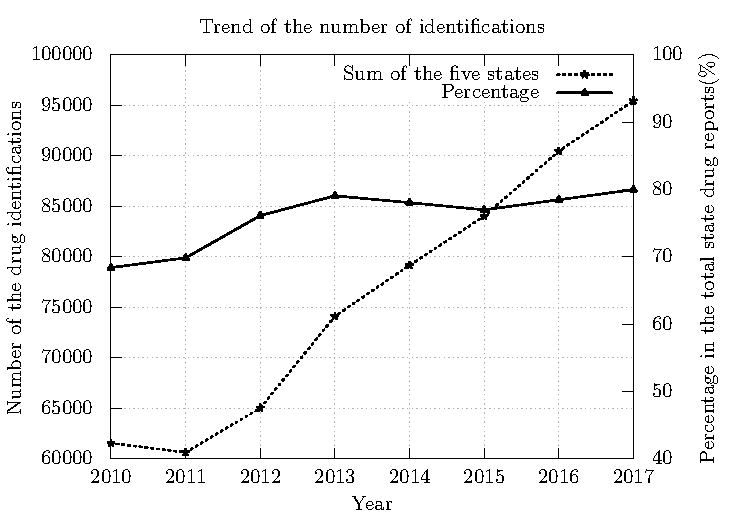
\includegraphics[width=10cm]{FiveStates.pdf}
  \caption{Trend of number of identifications}\label{1}
\end{figure}

\subsection{Restatement of the problems}
In this essay, our team is required to:
\begin{itemize}
\item[I. ] \textbf{Build a mathematical model which can characterize the trend of the change of drug identification reports between and in states and counties.} We see a class as the unit of the object observed in the spatial perspective and year in the temporal perspective and at last tell what the likeliest origin of the drug abuse is. Determination of classes will be done in pre-work. We will also answer the future concerns and their thresholds. The existing spatiotemporal sequences data of opioid drug reports is the only resource till now.
\item[II. ] \textbf{Combine socio-economic data provided with the model we have.} (As it is reasonable to believe socio-economic conditions have an intrinsic influence) Using this model, we can explain or verify some hypotheses about the level, objective, growth, and cause of the opioid drug abuse.

\item[III. ] \textbf{Apply our model to real-world issues and figure out some reasonable strategies to clamp down on the illegal circulation of the drugs.} We will test if they can work based on modifying our existing model with related factors then make suggestions.

\end{itemize}
Also, we focus exclusively on the test of any quantitative results to ensure their value to us.

\subsection{Pre-work}
\subsubsection{Qualitative analysis}
We think location information is essential in problems with prominent spacial features like propagation models. So we use the county-position list (attach each county with longitude \& latitude) by a crawler to build a time-series dynamic heat map about summed opioid drug reports to see what happens approximately (The deeper color an area has, the more reports there are):

\begin{figure}[htbp!]
  \begin{flushleft}
  	\begin{minipage}[t]{0.3\textwidth}
  \centering
  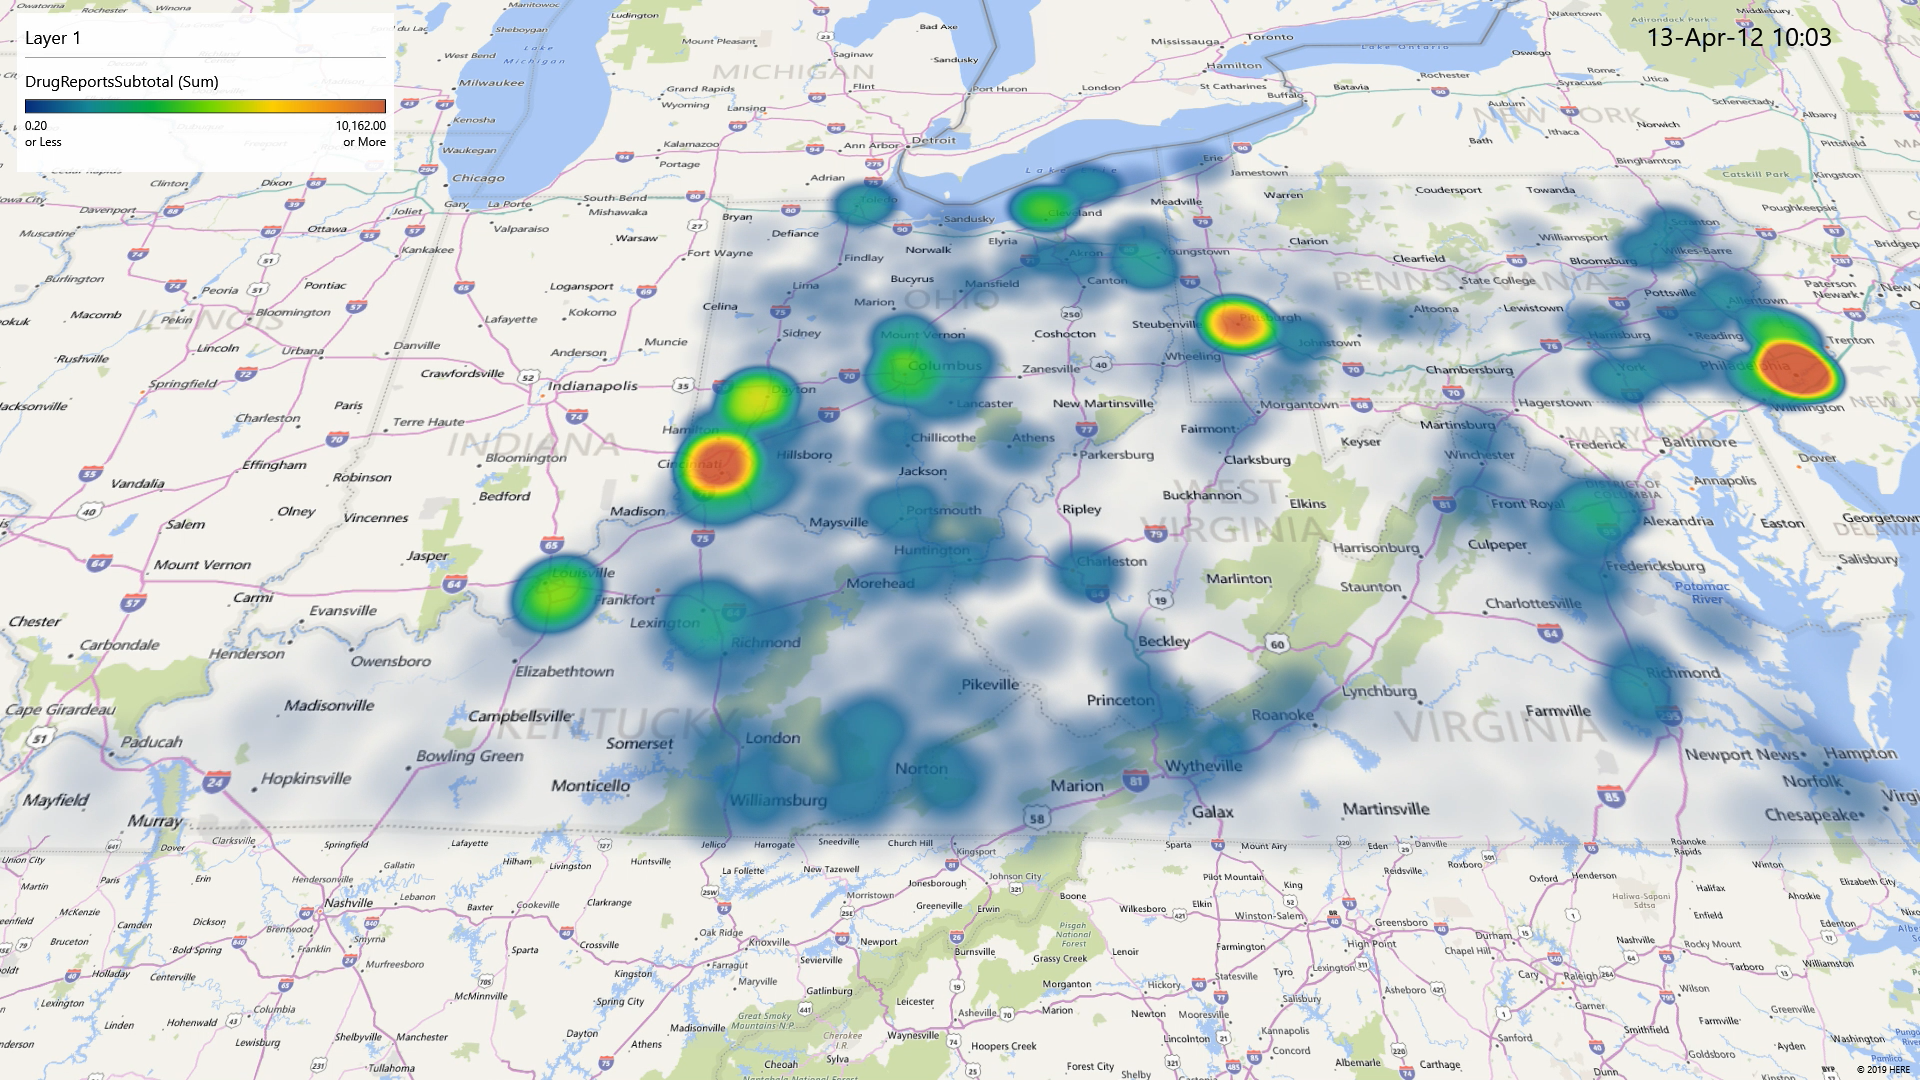
\includegraphics[scale=0.1]{s1.png}
  \caption{Heat map of the drug report in 2012}\label{2}
  \end{minipage}
  \qquad\qquad\qquad\qquad
  	\begin{minipage}[t]{0.3\textwidth}
  \centering
  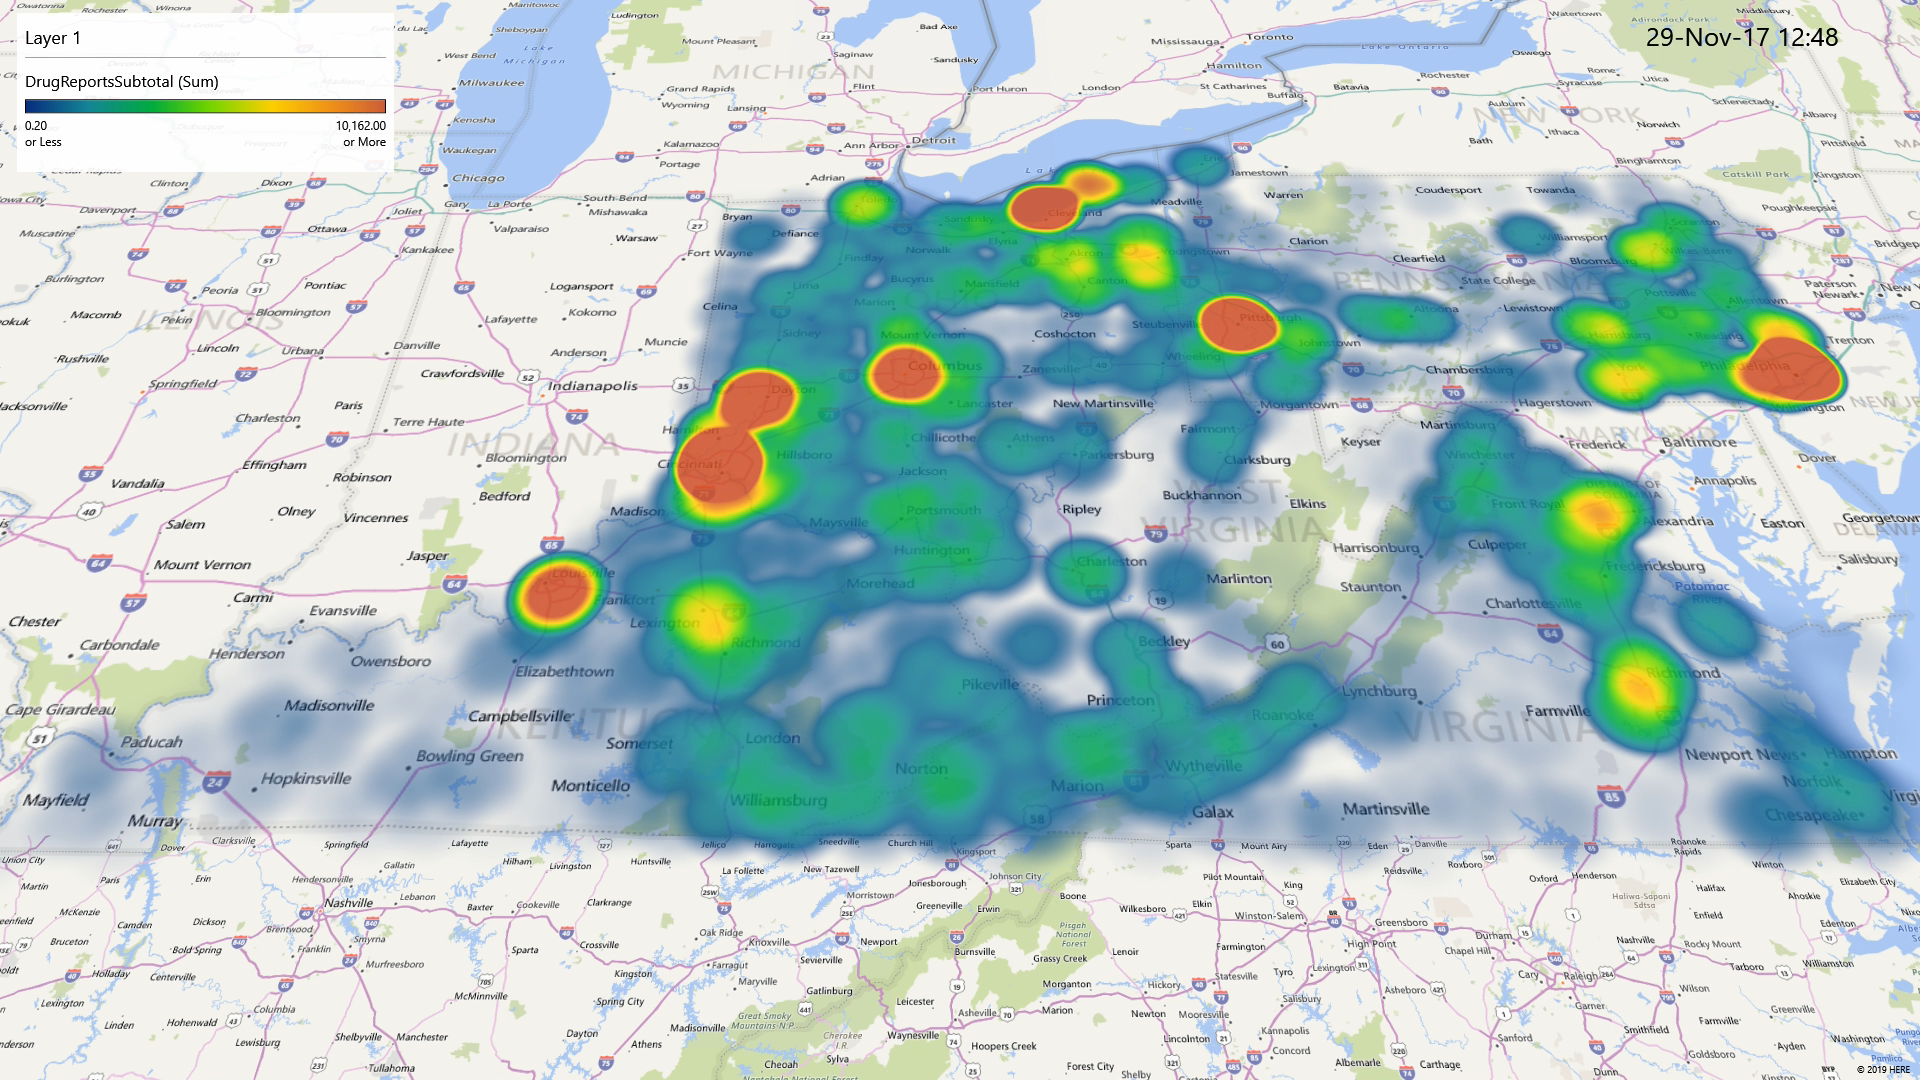
\includegraphics[scale=0.1]{s2.png}
  \caption{Heat map of the drug report in 2017}\label{3}
  \end{minipage}
  \end{flushleft}
  
\end{figure}

We can easily conclude that:
\begin{itemize}
	\item Counties with a large number of reports tend to keep fast growth of new opioid drug reports. The red-marked areas are always leaders of drug abuse.
	\item Counties with a large number of reports exert an enormous impact to its nearby areas. In other words, abuse-stricken areas have a constellation effect.
\end{itemize}
\subsubsection{Clustering before modeling}
Hence, clustering methodology is almost inevitable owing to features of the spread. We apply K-means (Stuart Lloyd, 1957) clustering to the division of all the counties according to their location and the total number of drug identification incidents. We choose 30 as the number of classes to fit for the actual situation of the heat map.
K-means clustering analysis is widely for deciding the specific class one object is in with no divided training sets. It aims to partition n observations into k clusters in which each observation belongs to the cluster with the nearest mean. The main steps of it are:
\begin{itemize}
	\item[1. ] Choose $K=30$ objects randomly as the initial clustering center from all the counties.
	\item[2. ] Repeat Step 3 and 4 until no county are allocated to a different class or the clustering center almost keeps the same at the deviation level of a set threshold value.
	\item[3. ] Calculate the distance from these centers for each counties (We give a weight for the number of drugs $x^c_i$ by multiplying them with $10\%$ after several attempts with different proportion for clustering accuracy, then turn the distance into the easy-to-calculate Euclid Distance)
	\item[4. ] Calculate the specific position of 30 centers again for next calculation in Step 3.
\end{itemize}


\begin{figure}[htbp!]
  \centering
  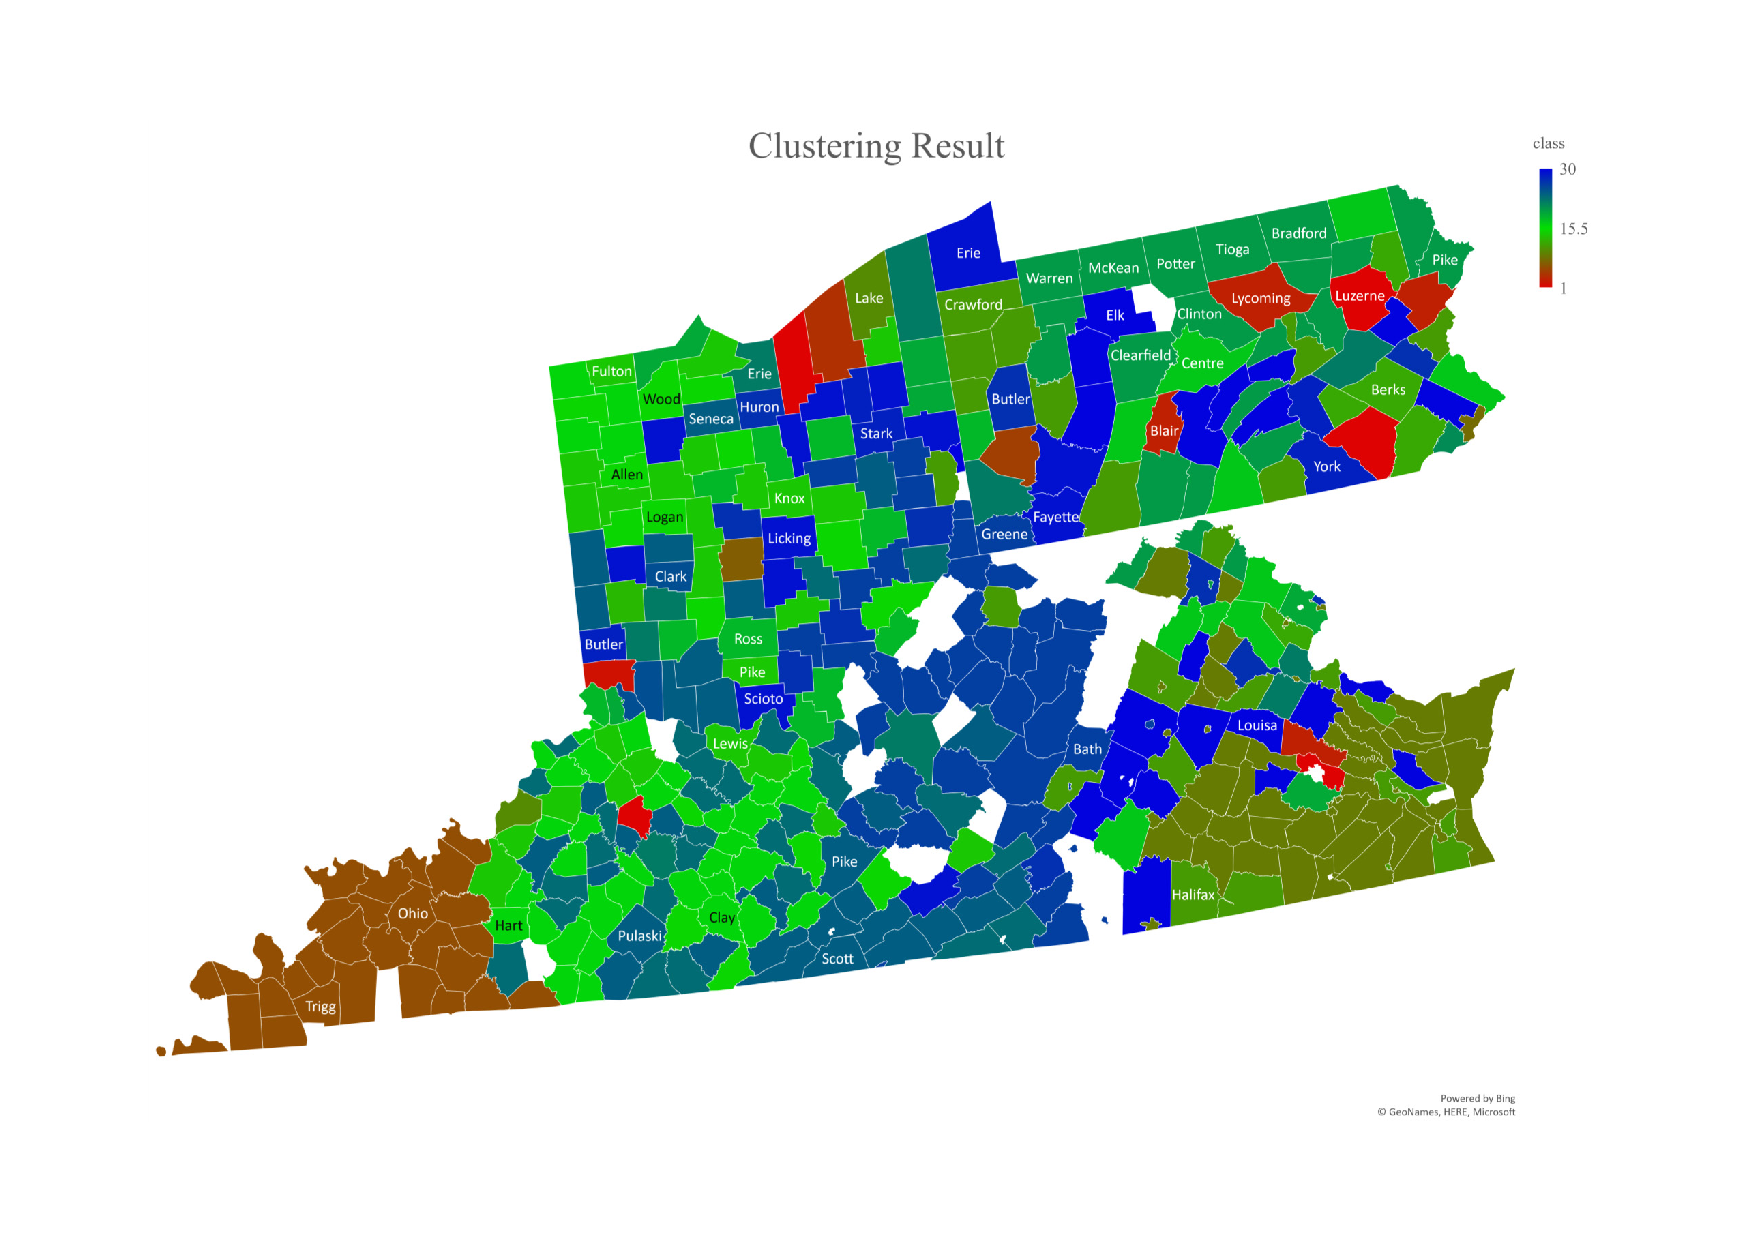
\includegraphics[width = 12 cm]{Clustering_3.pdf}
  \caption{The clustering result of the counties}\label{4}
\end{figure}


We generate 30 classes and set their position as the center of the in-class members. Now we have merged counties for reducing the calculating amount and eliminate random errors to a large extent according to the Law of Large Number. We think these groups have excellent properties in the sense of geography, traffic and opioid spread (Identity Assumption), which provides both facility and better results than merely considering the five states. Now we can base our research on these $30(class)*7(year)=210$ time-spacial series data item.

Matlab codes and specific clustering data for K-means are displayed in Appendix A. The clustering result is (Counties in each class share the same color):

\section{Notation}


\begin{tabular}{cp{0.8\textwidth}}
\toprule
 Symbols & Description\\
\midrule
 $x_i$ & Longitude \& latitude vector of clustering class $i$\\
 $y_{i,k}$ & Opioid drug reports of Class $i$ at a certain year ($k=year-2010$) \\
 $y^e_{i,k}$ & Estimated opioid drug reports of Class $i$ at a certain year ($k=year-2010$) \\
 $x^c_i$ & Latitude vector of County $i$ \\
 $t$ & Time (year as the unit, ranging from $0$ to $7$) \\
 $n_i$ & Total population of Class $i$\\
 $n^{'}_{i}$ & Rough total population of Class $i$\\
 $rep_{i}$ & Total drug reports of Class $i$\\
 $r_{ij}$ & The distance between the centers of Class $i$ and Class $j$\\
 $\lambda$ & The probability of a susceptible individual becoming a drug user after meeting  one\\
 $\alpha$ & The proportion of drug users who enter treatment and recover\\
 $\beta$ & The decay factor factoring when considering other classes\\
 $S_k(t)$ & The ratio of abuse susceptible individuals in the area of Class $k$. \\
 $I_k(t)$ & The ratio of drug users in the area of Class $k$. \\$R_k(t)$ & The ratio of individuals who already recovered in the area of Class $k$. \\
 $\Phi_k(t)$ & The formal ratio of drug users in the area of Class $k$ added by discounting weight of other classes. \\
 $\omega_{ij}$ & The drug abuse cultural exports weighting ratio of Class $i$ over Class $j$\\
 $Q$ & The relative residue between estimated and true new drug reports considering all years and classes\\
 $c_{ki}$ &The Criterion $i$ value of Class $k$\\
 $s_{ki}$ &The standardized Criterion $i$ value of Class $k$\\
 $re_{ij}$ & Correlation coefficient of Criterion $i$ and $j$\\
 $\beta i$ & Criterion $i$ that stands the test of the PSM-DiD method, $i=1,2,3,4$\\
 $score_{k,i}$ & The score of Class $k$ for Criterion $i$\\
 
 
\bottomrule
\end{tabular}
\section{Assumption \& Explanation}
\begin{itemize}
	\item  \emph{Identity Assumption: We recognizes counties in the same class as a whole and treat them as a single operational system.}  
	
	\small{Counties in the same class have high degree of similarity in location \& number of opioid drug reports. Between-class distances are considered.}
	\item \emph{Mobility Assumption: Transportation between states and counties are free. No  large-scale migration happens.} 
	
	\small{We rationalise the discounting factor based on this statement.}
	\item \emph{Model Idealization Assumption: Few (regarded as zero) people died unnaturally for abusing opioid drugs; Total population never changes a lot and drug users remains tiny at the period investigated.}
	
	\small{These conditions are suited for our modified model and we accept them because they are not too weird.}
	\item \emph{Moderate Policy Assumption: No state or county distinctly over-perform / underperform what they should be according to socio-economy conditions.}
	
	\small{It is the basis of our analysis of problem II and III using only the given data.}
	\item \emph{Socio-economy Stability Assumption: Data reflecting the socio-economy condition of each class remains stable during the year period.}
	
	\small{Thus we can tell the socio-economy condition choose any multiple criterion by just analyzing one year's annual socio-economy report. Actually, the data given cannot reject the assumption.}
\end{itemize}




\section{An double-modified SIR model}
\subsection{Model Overview}
First, we introduce the Susceptible Infected Recovered (SIR) Model to explain the spreading characteristic of the opioid drug abuse. We do not consider the proportion of people cured relapsing to drug users, as relapsing can be equally seen as uncured. Then we double-modify the model by adding the influence of other 29 classes to each class by using the cultural exports factor $\omega_{ij}$ and the discounting factor $e^{-\beta r_{ij}}$, where $\beta$ is the decay factor.

Having drawn the state transition model, we can write the corresponding differential equations naturally and give a numerical solution. At last, we refer to some essays and find the model's theoretical threshold considering the designed discounting factor. 

The rest work is to find the best parameters, where MATLAB offers available tools. When jumping ahead a particular time, we can see the class —— the origin of opioid drug abuse —— whose number of reports remains positive when others almost hit zero. 

The case of heroin is almost the same.
\subsection{Establishment \& Threshold Analysis}
Our team finds the heat map reveals plenty of physical features from qualitative analysis, so  any data-driven method that ignore the intrinsic characteristic may not work as well as a mechanism model (We will show this later).  Also, simple linear or logistic regression cannot keep robust on the long-term forecast. On the premise that drug use follows a process modeled in a similar way to the modeling of disease, we introduce SIR model (Kermack \& McKendrick, 1927) to see if the model yield insights on the spread. SIR model consists of three parts —— S for the number susceptible, I for the number of infectious, and R for the number recovered. 

Generally, we plot the transition model as:
\begin{figure}[htbp!]
\centering
	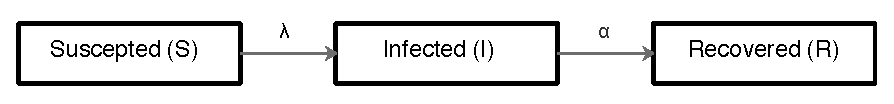
\includegraphics[width=12cm]{figures/SIR}
	\caption{The SIR model diagram}
\end{figure}

$\lambda$, $\alpha$, and $\beta$ are all transition rates from the corresponding two states (clear definition given in \textbf{Notation}). We consider $S(0)\approx1$ then the equation can be easily derived thus:
\[\begin{cases}
\tfrac{dS}{dt}= & -\lambda IS\\
\tfrac{dI}{dt}= & \lambda IS-\alpha I\\
\tfrac{dR}{dt}= & \alpha I
\end{cases} \]
where $S(0)=S_0\approx1,I(0)=I_0\approx0,R(0)=0, S(t)+I(t)+R(t)\equiv 1$.

For example, let $\alpha=0.1$, when $\lambda$ is ranging from $0.01$ to $0.2$ (step size is $0.005$). The graph is (lower $\lambda$ corresponds to lower curve):
\begin{figure}[htbp!]
	\centering
	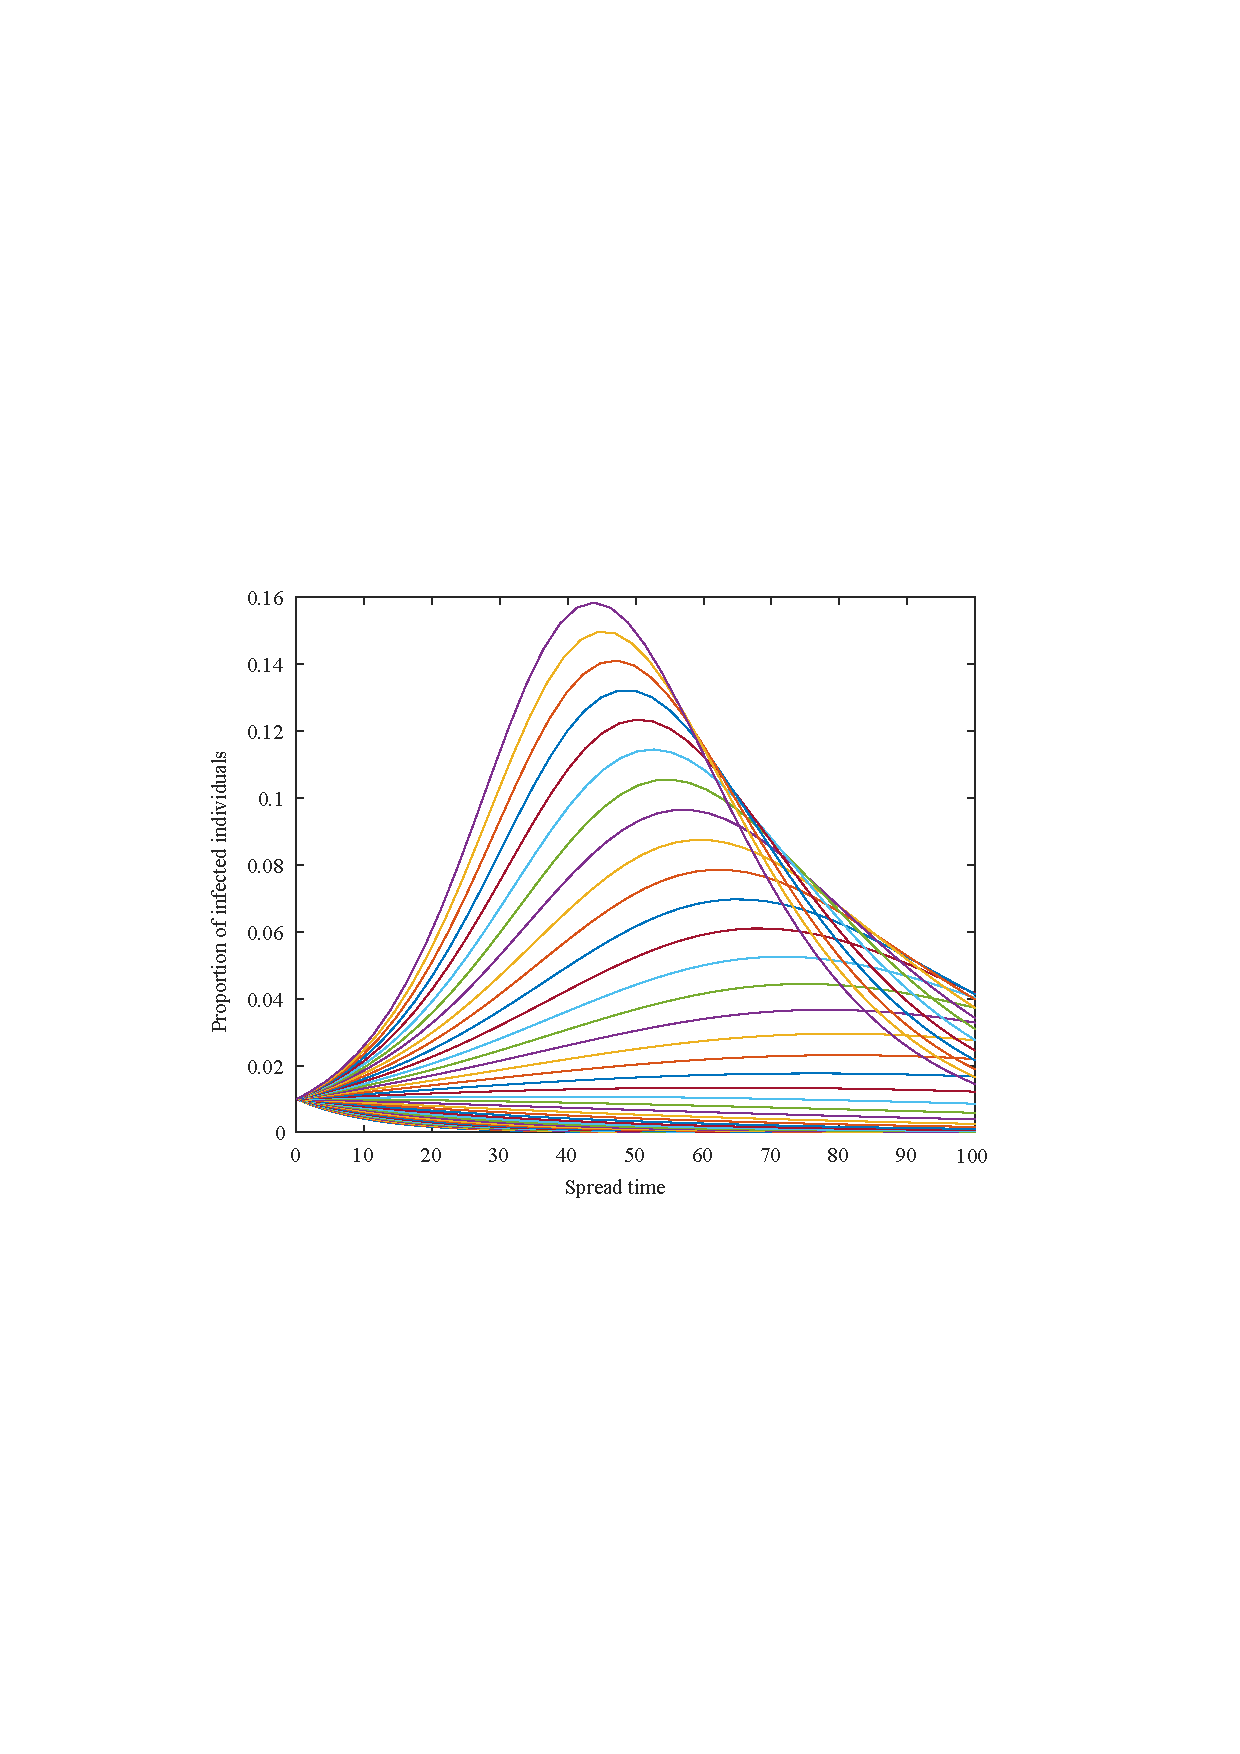
\includegraphics{SIRpdf}
	\caption{A demonstration graph for SIR model}
\end{figure}


The only controversial part is $IS$ in the model. It means the number of new drug users is bilinear to $I$ and $S$. We know that infections may achieve saturation and cannot keep such bilinear relation when $I$ is large. However, based on the Model Idealization Assumption, we can safely make such an approximation.

We do not consider the proportion of people cured relapsing to drug users, as relapsing can be equally seen as uncured. Therefore, $\alpha$ refers to the relapse-free recovery rate.

The SIR model is not applicable any more because the system is a complicated network. Traffic factors will change the internal structure of vulnerability to drug abuse. So the model requires us to make a modification to fit for the influence of the whole network.

We introduce a decay discounting factor $e^{-\beta r_{ij}}$, where $\beta$ is a positive decay factor and $r_{ij}$ is the distance from Class $i$ and Class $j$. The Mobility Assumption enables us to depict the decay discounting factor suited for all the classes just in a simple form. 

Then the influence of Class $j$ to Class $i$ considering $I_j$ and the distance discount rate is $\omega_{jk}e^{-\beta r_{ij}}I_j$. $\omega_{jk}$ is the drug abuse cultural exports weighting ratio of Class $j$ over Class $k$. In this problem we simply let$$\omega_{jk}=\dfrac{rep_j}{rep_k},$$ where $rep_j$ means total drug reports across seven years of Class $j$.

So we can calculate $\Phi_k(t)$: formal ratio of drug users in the area of Class $k$, which takes in potential drug users affected by other classes. Obviously $\Phi_k(t)$ combines all $I_k, k=1,2,..,30$. 

Let's first consider it in another way:
$$\Phi_k(t)=\sum_{j=1}^{30}P(j|k)I_j,$$
where$P(j|k)$ is defined as the probability of one individual in Class $k$ beginning to abuse drugs caused precisely by cultural exports of Class $j$. Taking notice of $\sum_{j=1}^{30}P(j|k)=1$, we let
$$P(j|k)=\dfrac{\omega_{jk}e^{-\beta r_{jk}}}{\sum_{j=1}^{30}\omega_{jk}e^{-\beta r_{jk}}},$$
then
$$\Phi_k(t)=\sum_{j=1}^{30}\dfrac{\omega_{jk}e^{-\beta r_{jk}}}{\sum_{j=1}^{30}\omega_{jk}e^{-\beta r_{jk}}}I_j$$

The modified model is depicted as:

\begin{figure}[htbp!]
	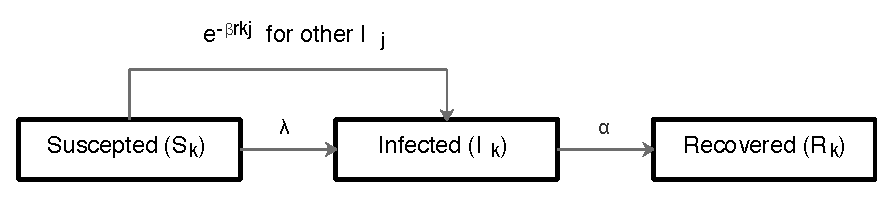
\includegraphics{figures/SIR2}
	\caption{Modified SIR model diagram}
\end{figure}

Corresponding equations are:
\[\begin{cases}
\tfrac{dS_k}{dt}= & -\lambda \Phi_k S_k\\
\tfrac{dI_k}{dt}= & \lambda \Phi_k S_k-\alpha I_k\\
\tfrac{dR_k}{dt}= & \alpha I_k
\end{cases} \]
where $S_k(0)=S_{k,0}\approx1,I_k(0)=I_{k,0}\approx0,R_k(0)=0$. 

The model establishment is completed.

Let the solution of $S_k$ be $S_k(t;I_{k,0})$ where $I_{k,0}$ is the initial value of $I_k$. We know that $I_{k,0}\ll1$. Due to the continuity of solution for an ordinary differential equation set to initial value, when 
$$I_{k,0}\rightarrow 0,$$
we have
 $$S_k(t;I_{k,0})\rightarrow s_k(t)=S_k(t;0)=e^{-\lambda\int_{0}^{t} \Phi_k(t)\, dt}$$
 Denote $\int_{0}^{t} \Phi_k(t)\, dt$ using $\phi_k(t)$. If we can stabilise the situation of the drug abuse, which means$$I_k(\infty)=0$$ for $k=1,2,..,30$, then $$R_k(\infty)=1-s_k(\infty)$$,so
 \begin{equation}
 	\begin{aligned}
 		\phi_k(t)&=\int_{0}^{t} \Phi_k(t)\, dt\\
 		&=\dfrac{\sum_{j=1}^{30}P(j|k)R_j}{\alpha}
 	\end{aligned}
 \end{equation}
 now we obtain
 \begin{equation}
 	\begin{aligned}
 		\phi_k(\infty)&=\dfrac{1-\sum_{j=1}^{30}P(j|k)e^{-\lambda\phi_j(\infty)}}{\alpha}\\
 		&=\dfrac{1-\sum_{j=1}^{30}\dfrac{\omega_{jk}e^{-\beta r_{jk}}}{\sum_{j=1}^{30}\omega_{jk}e^{-\beta r_{jk}}}e^{-\lambda\phi_j(\infty)}}{\alpha}
 	\end{aligned}
 \end{equation}

 
 We have learnt from some essays that $\phi_k(\infty)$ always exists. To get a untrivial solution of the equation above. We set $\phi_k(\infty)$ as the only argument now. In this way, the derivative of right hand side (RHS) at zero must be:
$$\dfrac{d}{\phi_k(\infty)}\dfrac{1-\sum_{j=1}^{30}\dfrac{\omega_{jk}e^{-\beta r_{jk}}}{\sum_{j=1}^{30}\omega_{jk}e^{-\beta r_{jk}}}e^{-\lambda\phi_j(\infty)}}{\alpha}|_{\phi_k(\infty)=0}>1.$$
Simplify it and we get the threshold:$$\dfrac{\lambda}{\alpha}>\sum_{j=1}^{30}\omega_{jk}e^{-\beta r_{jk}}.$$

The left hand side (LHS) remains a const when parameters are decided. So what we should do is only to calculate RHS and compare both side.

Now we get the theoretical threshold condition:
if the threshold condition above is satisfied, the ratio of drug abuse individuals in Class $k$ will remain at a positive level, which is dangerous and harmful to the society. The final stable level is the solution $x$ for Equation $x=\dfrac{1-\sum_{j=1}^{30}\dfrac{\omega_{jk}e^{-\beta r_{jk}}}{\sum_{j=1}^{30}\omega_{jk}e^{-\beta r_{jk}}}e^{-\lambda x}}{\alpha}.$ Otherwise, the trend will disappear even without any interference.
\subsection{Numerical Simulation \& Interpretation}

As we say at the last subsection, the cultural exports ratio $\omega_{ij}$ is denoted by $\frac{rep_i}{rep_j}$. The last thing we should do is the determination of the initial proportion of drug users $I_{k,0}$. Due to lack of data of the total population of every class, we give an estimation of $15*rep_k$ after brainstorm for the total population of Class $k$. Now we can eventually do the numerical simulation to get the value of $\lambda,\alpha,$ and $\beta$. Since our model is mechanical and the clustering in pre-work eliminate randomness to a large extent (thanks to Law of Large Number), we have reasons to believe our result \& estimation will be a proper one.

Before calculating the numerical solution, we claim that the ratio of new drug reports to the total population at time $t+1$ is:
\begin{equation}
 	\begin{aligned}
 		E_{kt}&=\quad \int_{t-1}^{t} \lambda \Phi_k S_k\, dt\\
 		&=\int_{t-1}^{t} (\dfrac{dI_k}{dt}+\alpha I_k)\, dt\\
 		&=I_k(t)-I_k(t-1)+R_k(t)-R_k(t-1)
 	\end{aligned}
 \end{equation}

We find the best value of $\lambda,\alpha,$ and $\beta$ so that $y^e_{k,t}=n^{'}_{i}(I_k(t)-I_k(t-1)+R_k(t)-R_k(t-1))$ is closest to the true value (new opioid drug reports). The definition of "closest" is relative residue between estimated and true new drug reports every year. When we achieve the minimum of relative residue 
$$\min \limits_{\lambda, \alpha, \beta} Q=\dfrac{\sum_{k=1}^{30}\sum_{t=1}^{7}\frac{y^e_{k,t}-y_{k,t}}{y_{k,t}}}{210},$$
the parameters are the best.

The Matlab codes for the ODE numerical solutions are in Appendix C. Because drawing all 30 classes dazzles eyes much, we just pick three of them as a representative set. Different kinds of line styles indicate different classes:
\newpage
\begin{figure}[htbp!]
  \begin{flushleft}
  	\begin{minipage}[t]{0.3\textwidth}
  \centering
  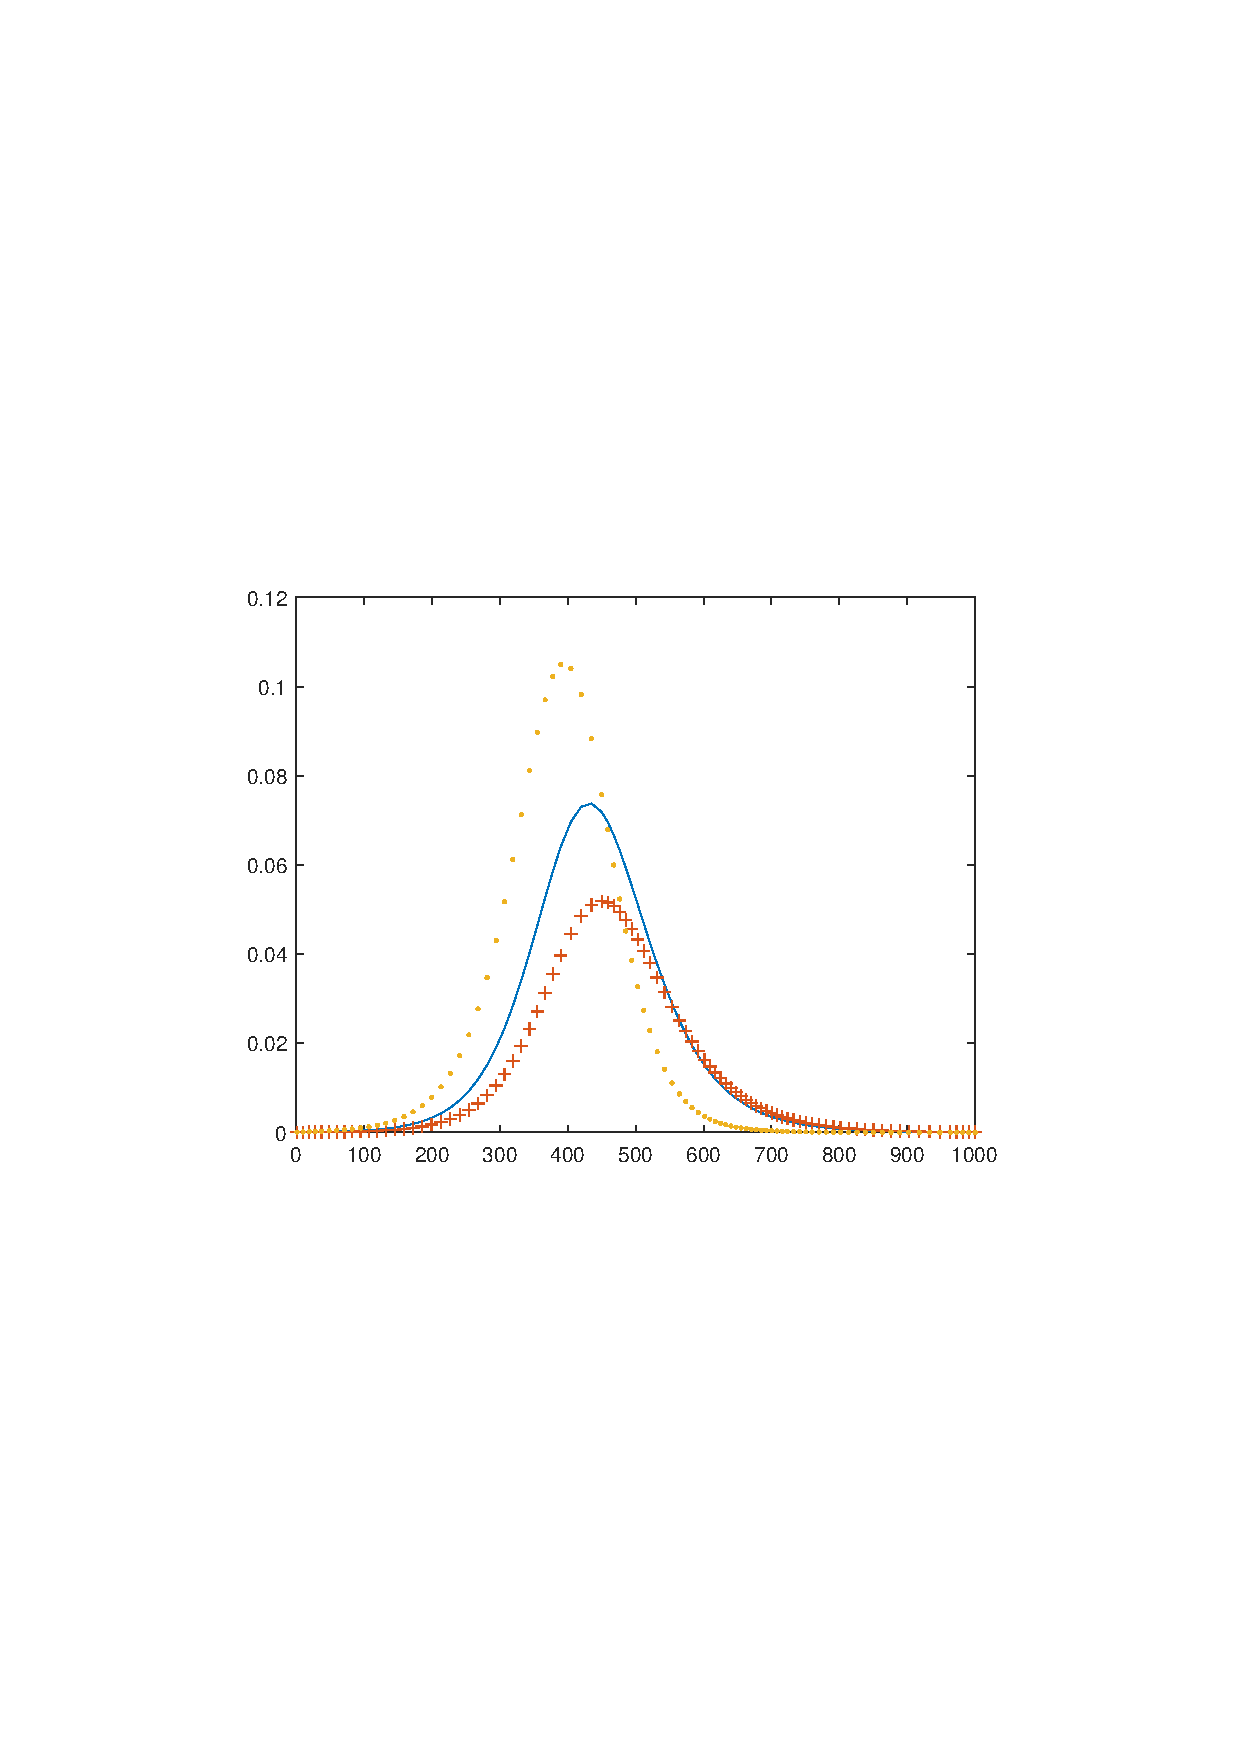
\includegraphics[width=8cm]{/figures/f1}
  \caption{Graph when $\lambda=0.05$, $\alpha=0.03$, $\beta=0.1$, Dependent variable: $I$}
  \end{minipage}
  \qquad\qquad\qquad\qquad
  	\begin{minipage}[t]{0.3\textwidth}
  \centering
  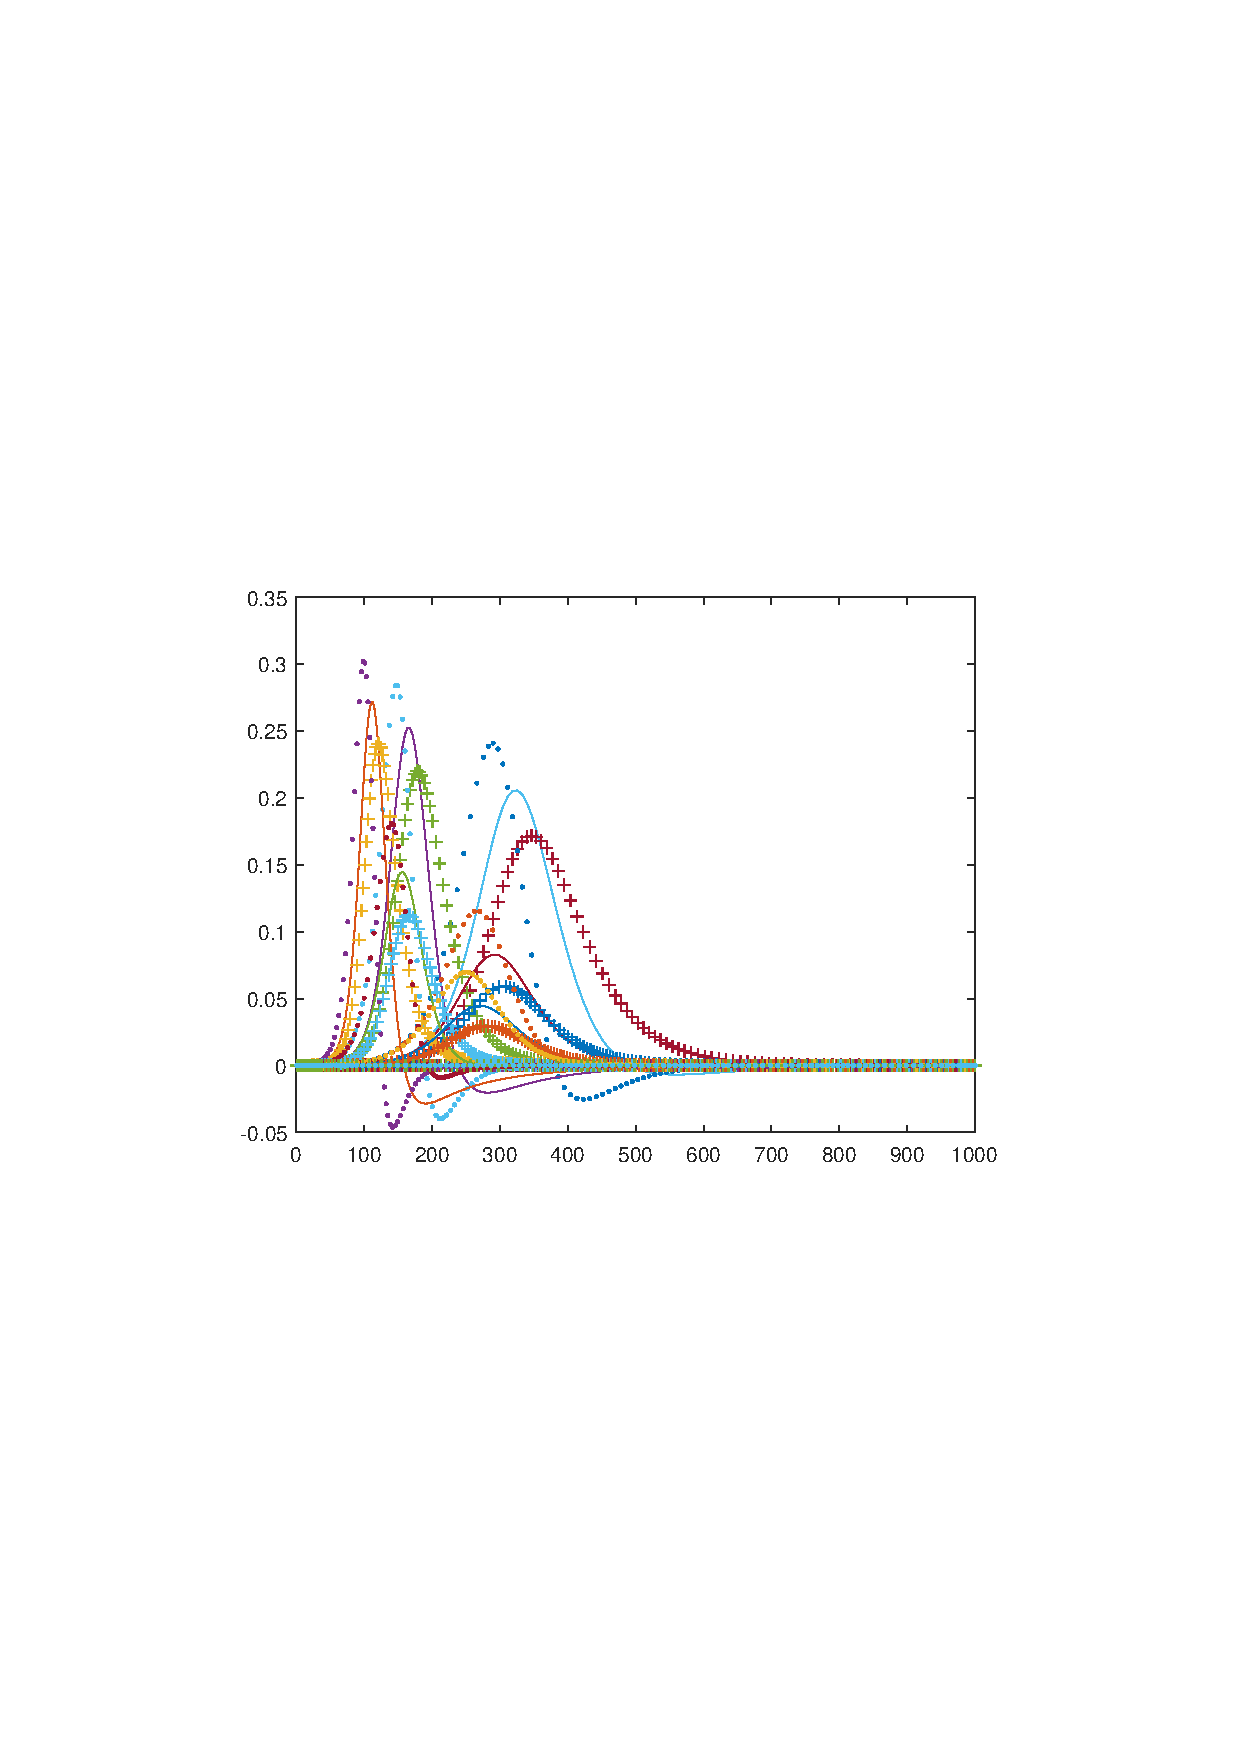
\includegraphics[width=8cm]{/figures/f2}
  \caption{Graph when $\lambda$ and $\alpha$ changes, $\beta=0.098$, Dependent variable: $I$}
  \end{minipage}
  \end{flushleft}
  
\end{figure}


We then run the procedure and get when the relative residue $Q$ is the smallest:
$$\lambda=0.011 \qquad \alpha=0.077 \qquad \beta=0.098, \qquad Q=0.01$$ the results are pretty much in line with our expectations that both $\lambda$ and $\alpha$ will be small and $\beta$ will not be that big because when we manually set decaying factor $\beta$ over 5, the graph almost did not show changes under the pressure of the network effect. The $Q$ meets the I Accuracy level, so our model is quite explainable for the spread. 

The graph of the best parameters is:

\begin{figure}[htbp!]
  \begin{flushleft}
  	\begin{minipage}[t]{0.3\textwidth}
  \centering
  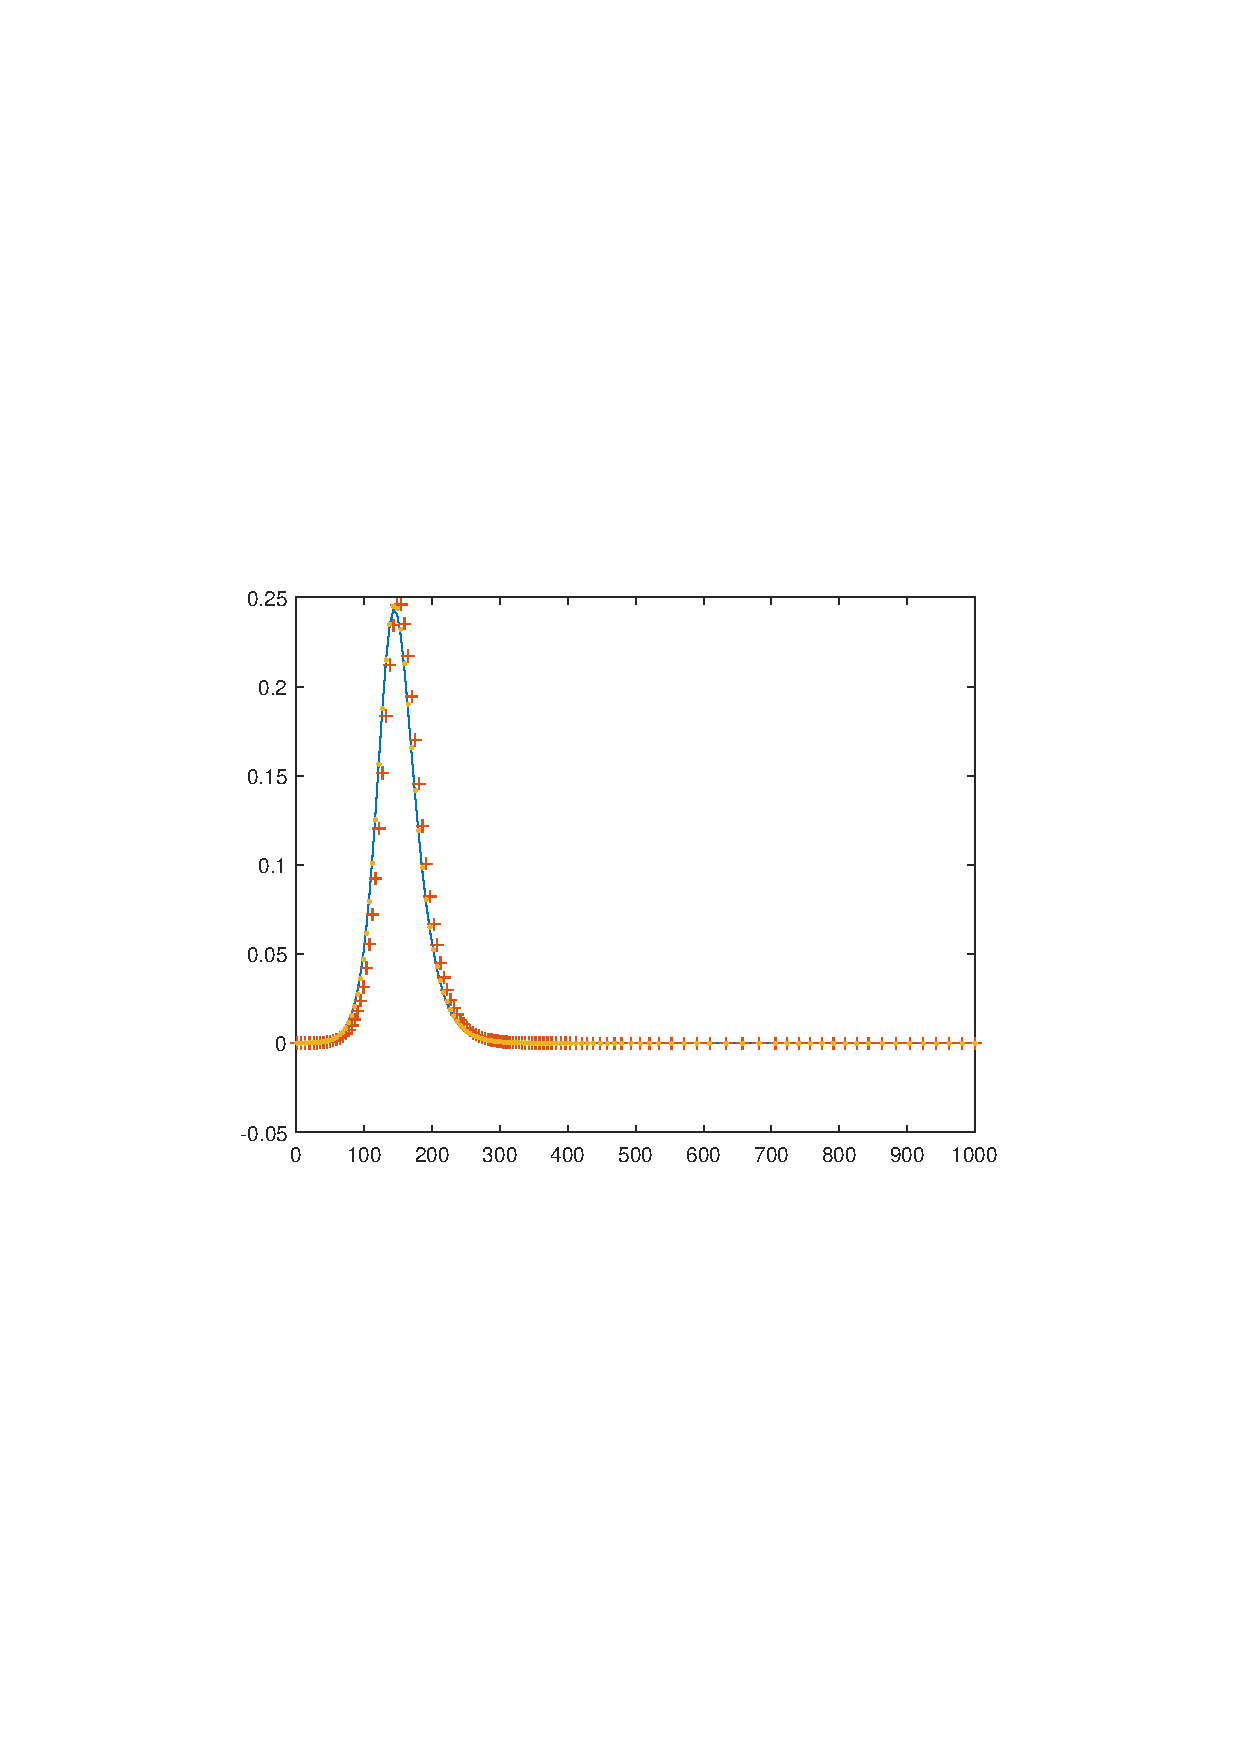
\includegraphics[width=8cm]{/figures/f4}
  \caption{Best parameters, Dependent variable: $I$}
  \end{minipage}
  \qquad\qquad\qquad\qquad
  	\begin{minipage}[t]{0.3\textwidth}
  \centering
  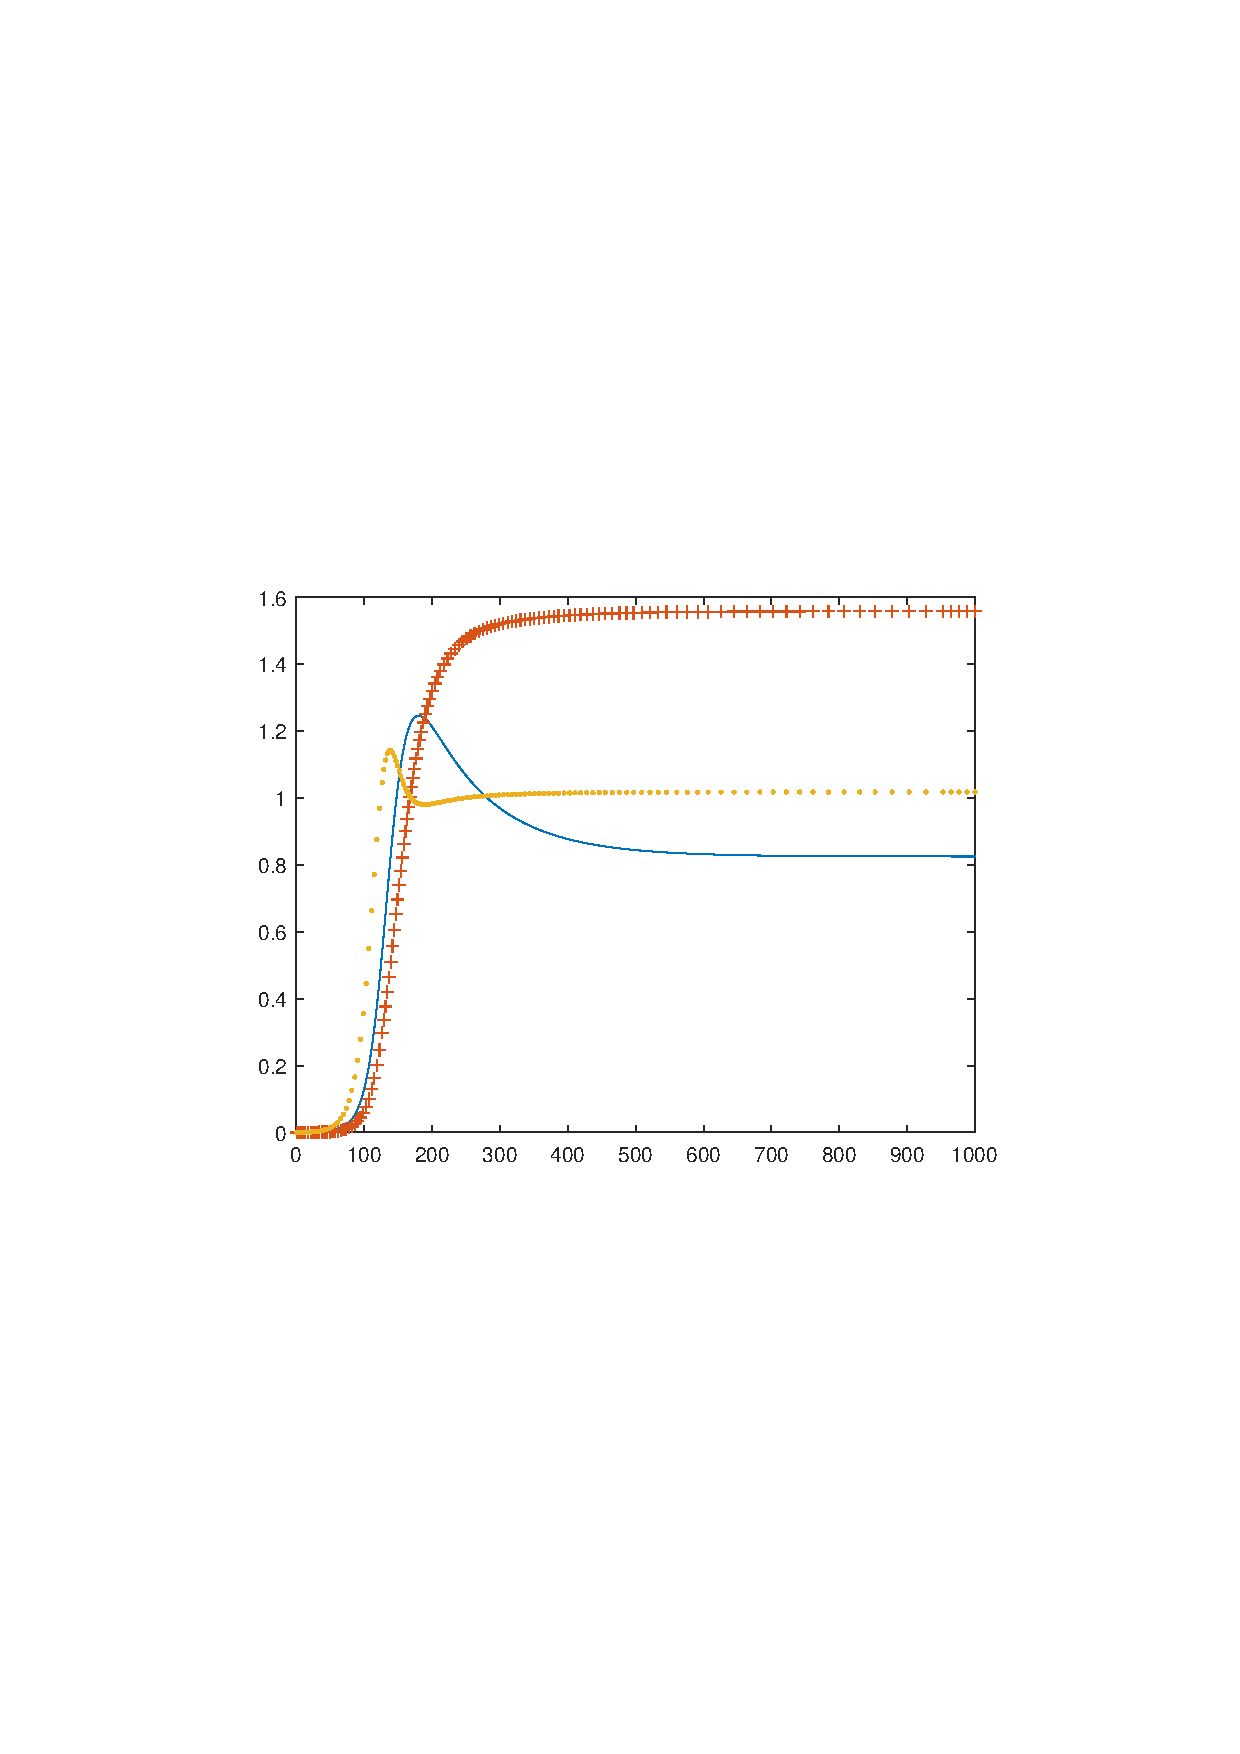
\includegraphics[width=8cm]{/figures/f3}
  \caption{Best parameters, Dependent variable: $I+R$}
  \end{minipage}
  \end{flushleft}
  
\end{figure}

As to the Heroin, since $\beta$ is an objective parameter which is decided by the road condition, it is fixed to $\beta=0.098$. The best parameters is:
$$\lambda=0.010, \alpha=0.053$$

To find the origin, we first classify the classes into 5 groups according the state they belong to. Then for classes in every group, we pull the time of the graph back for 5 years. The class whose time when the curve hit 0.00001\% the earliest is the likeliest origin. We then find Class is the possible origin. By analyzing the heat map of each county in the 5 classes, we figure out \textbf{Jefferson, Kentucky (Class 10); Hamilton, Ohio (Class 2); Philadelphia, Pennsylvania (Class 8); Monongalia, West Verginia (Class 26)} are the most possible origins of Heroin.

The trend and characteristic are prominent now: it keeps growing linearly approximately, but at a certain point-in-time it will boost into a high peak. Also, this point-in-time of drug gathering places will be earlier for 5-10 years. Though no class surpasses the threshold, the peak of 15-30\% is quite scaring.

Our model tells us that the United States are facing severe challenges. Without interfere,  the drug abuse will fully break out in \textbf{40-50} years. I think the point-in-time will be \textbf{earlier} in reality because people will be in closer and closer contact with each other ($\lambda$ is not static for the long term!) We must take action to solve the problem. 



\section{Methods \& Models when processing lots of data}
\subsection{Model Overview}
We at first preprocess the data by ticking column with all zeros and part of elements lost. We also standardize each column of data for better analysis (like PCA methods).

To find the influential factors, we employ the Principal Component Analysis (PCA) to find objective criteria to simplify the data. Also, we manually add some subjective criteria like Education and Marital with Analytic Hierarchy Process (AHP) evaluation model. As we now get many criteria, we test if they continue influencing opioid drug reports by a statistical method PSM-DiD. 

We try to make our former model become more and more robust and precise using the data we get.  To add the factors to our double-modified SIR model, we first the result tells which criterion is efficient via our former work above. Then we can modify the origin model by letting some parameters be the non-const function of these criteria. Finally, we see if the model now gives a better estimation.
\subsection{Establishment \& Analysis}
We tick away the criterion columns with default value or with all zeros (all zeros have no information). We do not consider the Margin of Error columns because the level of error is not high.

We make a standardized processing then. For each criterion value (Column $i$, Class$k$) $c_{ki}$, we let:
$$s_{ki}=\dfrac{c_{ki}-\overline{c}_i}{\sqrt{Var(\overline{c}_i)}}$$
Here $Var(\overline{c}_i)$ means sample variance of Column $i$. Now we get another useful table.
%=================================================
\subsubsection{Selection of Subjective \& Objective Indicators - AHP \& PCA}
The widely-acknowledged Analytic Hierarchy Process (AHP) Methods (Satty, 1971) turns the intangible criteria into tangible ones. It has a hierarchical structure with at least three levels.

\begin{figure}[htbp!]
\centering
	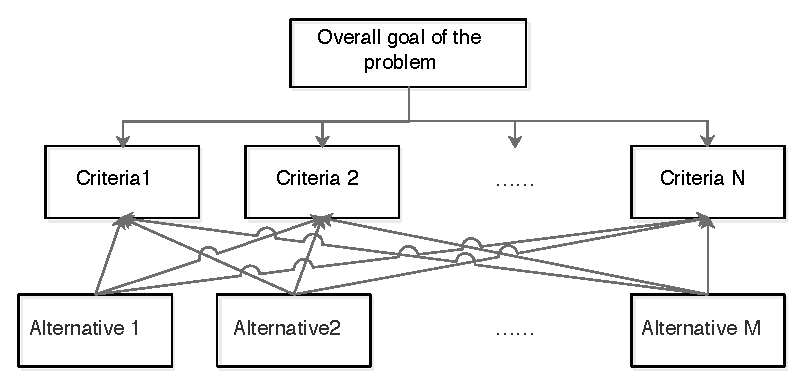
\includegraphics{1}
	\caption{Schematic diagram of the AHP method}
\end{figure}

Here alternatives refer to 30 classes. Our goal now is to find the weight of each criterion. For many hypotheses proposed, we analyze the different emphasis on education, households and population structure. We do so because Socio-economy Stability Assumption tells us all the selected criteria remain indicative all the time.

We first construct of the evaluation matrix $\mathbf{A}$ which determines the relative importance of the criteria:

\[ \mathbf{A} = \left(
\begin{array}{cccc}
a_{11} & a_{12} & \ldots & a_{1n}\\
a_{21} & a_{22} & \ldots & a_{2n}\\
\vdots & \vdots & \ddots & \vdots\\
a_{n1} & a_{n2} & \ldots & a_{nn}\\
\end{array} \right) \]
We have to claim that:
\begin{itemize}
	\item  Let it $C_i$ be criteria $i$, then $a_{ij} (i,j=1,2,..,n)$ means the ratio of the importance of $C_i$ and $C_j$
	\item It is clear that $a_{ii}=1, a_{ij}a_{ji}=1, a_{ii}\ne0$, and $a_{ji}=1/n$ indicates that the relation of importance is inverse to the former integer number $n$.
	\item To get the specific value of $a_{ij}$, we have a suggestion table for reference (Odd number means the importance between two neighbors):%
	\end{itemize}
	\begin{table}[!htbp]
  \small
  \centering
    \begin{tabular}{ccccccc}
    \toprule
    $a_{ij}$ & 1&3&5&7&9\\
    Meaning(importance) &Equal&Moderately more&More&Strongly more&Extremely more\\
   
    \midrule 
    \end{tabular}%
\end{table}%%%%%%%%%%%%%%%%%%%%%%%%%%%%%%%

As for the matrix $\mathbf{A}$, The eigenvectors corresponding to the biggest eigenvalue is the weight we want.

We consider education degree, dispersiveness of families, and well-being in marriage (Data in 2016). The result is (all of them undergo consistency tests, $CR<0.1$):
\begin{itemize}
	\item \textbf{Education:} HC01\_VC88, HC01\_VC89, HC01\_VC90, HC01, \_VC91, HC01\_VC96
	
		$$ \left(
\begin{array}{ccccc|c}
1 & 1/3 & 1/5 & 1/7 & 1/9 & 0.0435\\
3 & 1 & 1/3 & 1/6 & 1/9 & 0.0722\\
5 & 3 & 1 & 1/4 & 1/8 & 0.1370\\
7 & 6 & 4 & 1 & 1/7 & 0.3093\\
9 & 9 & 8 & 7 & 1 & 0.9373\\
\end{array} \right) $$

	\item \textbf{Households:} HC01\_VC03, HC01\_VC08, HC01\_VC11, HC01\_VC14, HC01\_VC21.	
	$$ \left(
\begin{array}{ccccc|c}
1 & 1/7 & 1/5 & 7 & 3 & 0.2166\\
7 & 1 & 7 & 9 & 5 & 0.9048\\
5 & 1/7 & 1 & 5 & 1/3 & 0.2707\\
1/7 & 1/9 & 1/5 & 1 & 1/7 & 0.0399\\
1/3 & 1/5 & 3 & 7 & 1 & 0.2438\\
\end{array} \right) $$

	\item \textbf{Marital:} HC01\_VC26, HC01\_VC38, HC01\_VC44, HC01\_VC45, HC01\_VC46
	$$ \left(
\begin{array}{ccccc|c}
1 & 5 & 1/7 & 4 & 1/5 & 0.1937\\
1/5 & 1 & 1/9 & 2 & 1/7 & 0.0756\\
7 & 9 & 1 & 6 & 3 & 0.8542\\
1/4 & 1/2 & 1/6 & 1 & 1/5 & 0.0711\\
5 & 7 & 1/3 & 5 & 1 & 0.4711\\
\end{array} \right) $$
\end{itemize}
Now we have got all subjective indicators.

Principal Component Analysis (PCA) method is used to reduce the complexity when we handle a lot of variables with complicated relationships inside them. We find several criteria which is uncorrelated and easier to analyze.

For the implementation method, first we calculate the correlation coefficient between all criteria and get the correlation coefficient matrix:
\[ \mathbf{R} = \left(
\begin{array}{cccc}
re_{11} & re_{12} & \ldots & re_{1n}\\
re_{21} & re_{22} & \ldots & re_{2n}\\
\vdots & \vdots & \ddots & \vdots\\
re_{n1} & re_{n2} & \ldots & re_{nn}\\
\end{array} \right) \]

Then we calculate the eigenvalues and eigenvectors of $\mathbf{R}$ and select eigenvectors whose eigenvalues are over 1 as the principal indicators. In our problem, Socio-economy Stability Assumption tells us principal indicators in one year are suited for all years. At last, we chose 6 principal indicators here.

We do the calculation using SPSS. The full result is in Appendix B (There are too many criteria).So far, we have got all the indicators we want to analyze whether they have influences on drug reports.
\subsubsection{Influential or Nothing? - PSM-DiD \& New Model}
The PSM-DiD method is a statistical model specially designed for judging whether a policy or an kind of essential difference will influence, no matter better or worse, the value we speculate. We call the essential difference 'external difference'. We take the economy level as an example.

Assume $D_i\in\{0,1\}$ means whether the area of a class has a good economy level. Better areas (the number is half of the total) are grouped into Treatment Group $D=1$. The others are grouped into Control Group $D=0$.$T_i\in\{0,1\}$ means two time periods (now we set it as 2010-2013 \& 2014-2017). Then the difference-in-difference is:
$$\Delta\Delta Y=(Y(T=1,D=1)-Y(T=0,D=1))-(Y(T=1,D=0)-Y(T=0,D=0)),$$
where $Y(T,D)$ means the total opioid drug reports of Group $D$ at time period $T$. If $\Delta\Delta Y$ is a number significantly large (sometimes $0.1\sum_{T,D}Y(T,D)$), we say the difference in economy does influence the opioid drug abuse positively (negatively if the sign symbol is "-").

That is a simpler version of what DiD does. But the problem is, there is 'internal difference' which disturbs our experiment. For example, maybe classes with better economy often have better education and it is education level that really affects the drug abuse. So we introduce PSM method to eliminate this error. The basic idea is, pair every class in Treat Group with a class whose criteria (except the economic ones) is quite close to it and thanks to the Law of Large Number, the experiment can be carried out with no internal difference. In this case, since a class has  invariability of the value's scale (One class whose all value of criteria is as twice as another one means their condition are almost the same), we utilize the vectorial angle to judge the 'close':
$$'close'degree (i \& j)=\dfrac{\sum_k c_{ik}*c_{jk}}{\mathbf{|c_i|*|c_j|}},$$
where $\mathbf{c_i}$ means the Euclid length of all the criteria of Class $i$. The closer degree of 'close' is to 1, the more similarity they have.

So we employ all 6 indicators generated by PCA and 3 indicators generated by AHP to see the PSM-DiD result $\Delta\Delta Y$. For each indicator, we find 10 classes with the best scores (that can be seen as a matrix multiplication) and find 10 pairs for each of them as the control group. We tick away their own ratio of corresponding criteria before calculating the vectorial angle (as to AHP indicators, we tick away all relevant criteria). 

We find only 4 indicators influences the result with statistical significance. By the way, the hypotheses about marriages can be rejected though it seems reasonable in some sense. It is quite surprising that higher education level an area has, the more opioid drugs people take. The result table is:

\begin{table}[htbp]
\centering
\begin{tabular}{p{90pt}<{\raggedright}lp{90pt}<{\raggedleft}p{90pt}<{\raggedleft}}
\toprule[1.5pt]
Indicator & Group & 2010-2013 & 2014-2017\\
\midrule[1pt]
 {\textcolor[rgb]{ 1,  0,  0}{Education}} & Treatment & 6990 & 8804 \\
 & Control & 5401 & 4033 \\
 {\textcolor[rgb]{ 1,  0,  0}{Households}} & Treatment & 3442 & 3998 \\
   & Control & 5023 & 3625 \\
   Marital & Treatment & 8146 & 8769 \\
     & Control & 4079 & 4451 \\
     PCA1 & Treatment & 6690 & 8804 \\
       & Control & 4485 & 4671 \\
       {\textcolor[rgb]{ 1,  0,  0}{PCA2}} & Treatment & 2770 & 9716 \\
        & Control & 4194 & 4670 \\
         PCA3 & Treatment & 8951 & 9909 \\
           & Control & 4125 & 4562 \\
           PCA4 & Treatment & 6316 & 7018 \\
            & Control & 5664 & 5445 \\
           PCA5 & Treatment & 3222 & 3839 \\
            & Control & 3270 & 2939 \\
           {\textcolor[rgb]{ 1,  0,  0}{PCA6}} & Treatment & 7745 & 9087 \\
            & Control & 4179 & 3203 \\
\bottomrule[1.5pt]

\end{tabular}
\caption{PSM-DiD testing for 9 indicators - Results} 
\end{table}

We let these 4 indicators be $\beta1,\beta2,\beta1,\beta3$ and $\beta4$ respectively. We let the score of Class $k$ for $\beta i$ be $score_{k,i}$ (We use the panel which is standardized). Since $\alpha$ and $\beta$ have nothing to do with the data we have. We try to modify our double-modified SIR model in three ways:
\begin{itemize}
	\item[I. ] More precise const: The total population is available so there is no need to use that rough estimator.
	\item[II. ] Personalized parameter: Variable $\lambda_k=f_{\lambda_k}(\beta1,\beta2,\beta3,\beta4)$. $\lambda$ is positively related to $\beta1,\beta2$ because we can assume that better education and more dispersal families lead to higher $\lambda$. We notice that designing $\lambda$ without using \textbf{the fundamental $\mathbf{\lambda}$ }in Problem I will make the parameter fluctuate to an abnormal.
	\item[III. ] More applicable parameter: Variable $\omega_{ij}=f_{\omega_{ij}}(\beta1,\beta3,\beta4,ttppl)$. $\omega$ is positively related to $\beta1$ and uncorrelated with $\beta 2$. Also, total population along with the number of drug reports will influence the cultural influence, but not that much.
\end{itemize}

We first calculate the best parameters using the more precise const —— "$I_{k,0}$", only to find the results remain almost the same. It verifies the continuity of solution for an ordinary differential equation set to initial value in a peculiar way. The construction of $\lambda$ and $\omega_{ij}$ functions are a quite complicated job with high technical content. Due to lack of time, we do not employ methods about any machine learning any more and give only two simple but reasonable estimators to inspire the readers:

$$\lambda_k=\lambda*(1+\sigma_5 score_{i,1}+\sigma_6 score_{i,3}+\sigma_7 score_{i,4})$$
$$\omega_{i,j}=\dfrac{rep_i*log(n_i)^{\sigma}*(1+\sigma_1 score_{i,1}+\sigma_2 score_{i,2})+\sigma_3 score_{i,3}++\sigma_4 score_{i,4}}{rep_j*log(n_j)^{\sigma}*(1+\sigma_1 score_{j,1}+\sigma_2 score_{j,2})+\sigma_3 score_{j,3}++\sigma_4 score_{j,4}}$$

By calculating the best parameters $\sigma$ and $\sigma_i, i=1,2,..,7$, we can lower $Q$ value in advance and give a better estimation. In this sense, A data-integrated SIR is completed. Whenever there is fresh data, we can combine them with our model using the same steps we do.

\textbf{For Part III,} we think the feasible strategy to hinder the drug abuse must satisfy little harm to the society. So blindly lowering the education level or force people to live together in order to decrease the value of $\lambda$ is ridiculous. After deliberation about both the model and the reality, we point out a less common principle:
\begin{center}
	Increase the cultural influence of the areas where the situation drug abuse is good.
\end{center}

The government can publicize the 'No-drug exemplary counties' to help make it. Also, we can encourage childbirth properly in these counties to increase the population. We can even develop local tourism to achieve our goal. Of course, there are many specific ways to do so.

We would like to share you a figure where we double the cultural influence of 5 classes in good condition by heightening some $\omega_{ij}$. The objects are three classes far away from the 5 classes mentioned above. ($\lambda=0.05, \alpha=0.03$)

\begin{figure}[htbp!]
  \begin{flushleft}
  	\begin{minipage}[t]{0.3\textwidth}
  \centering
  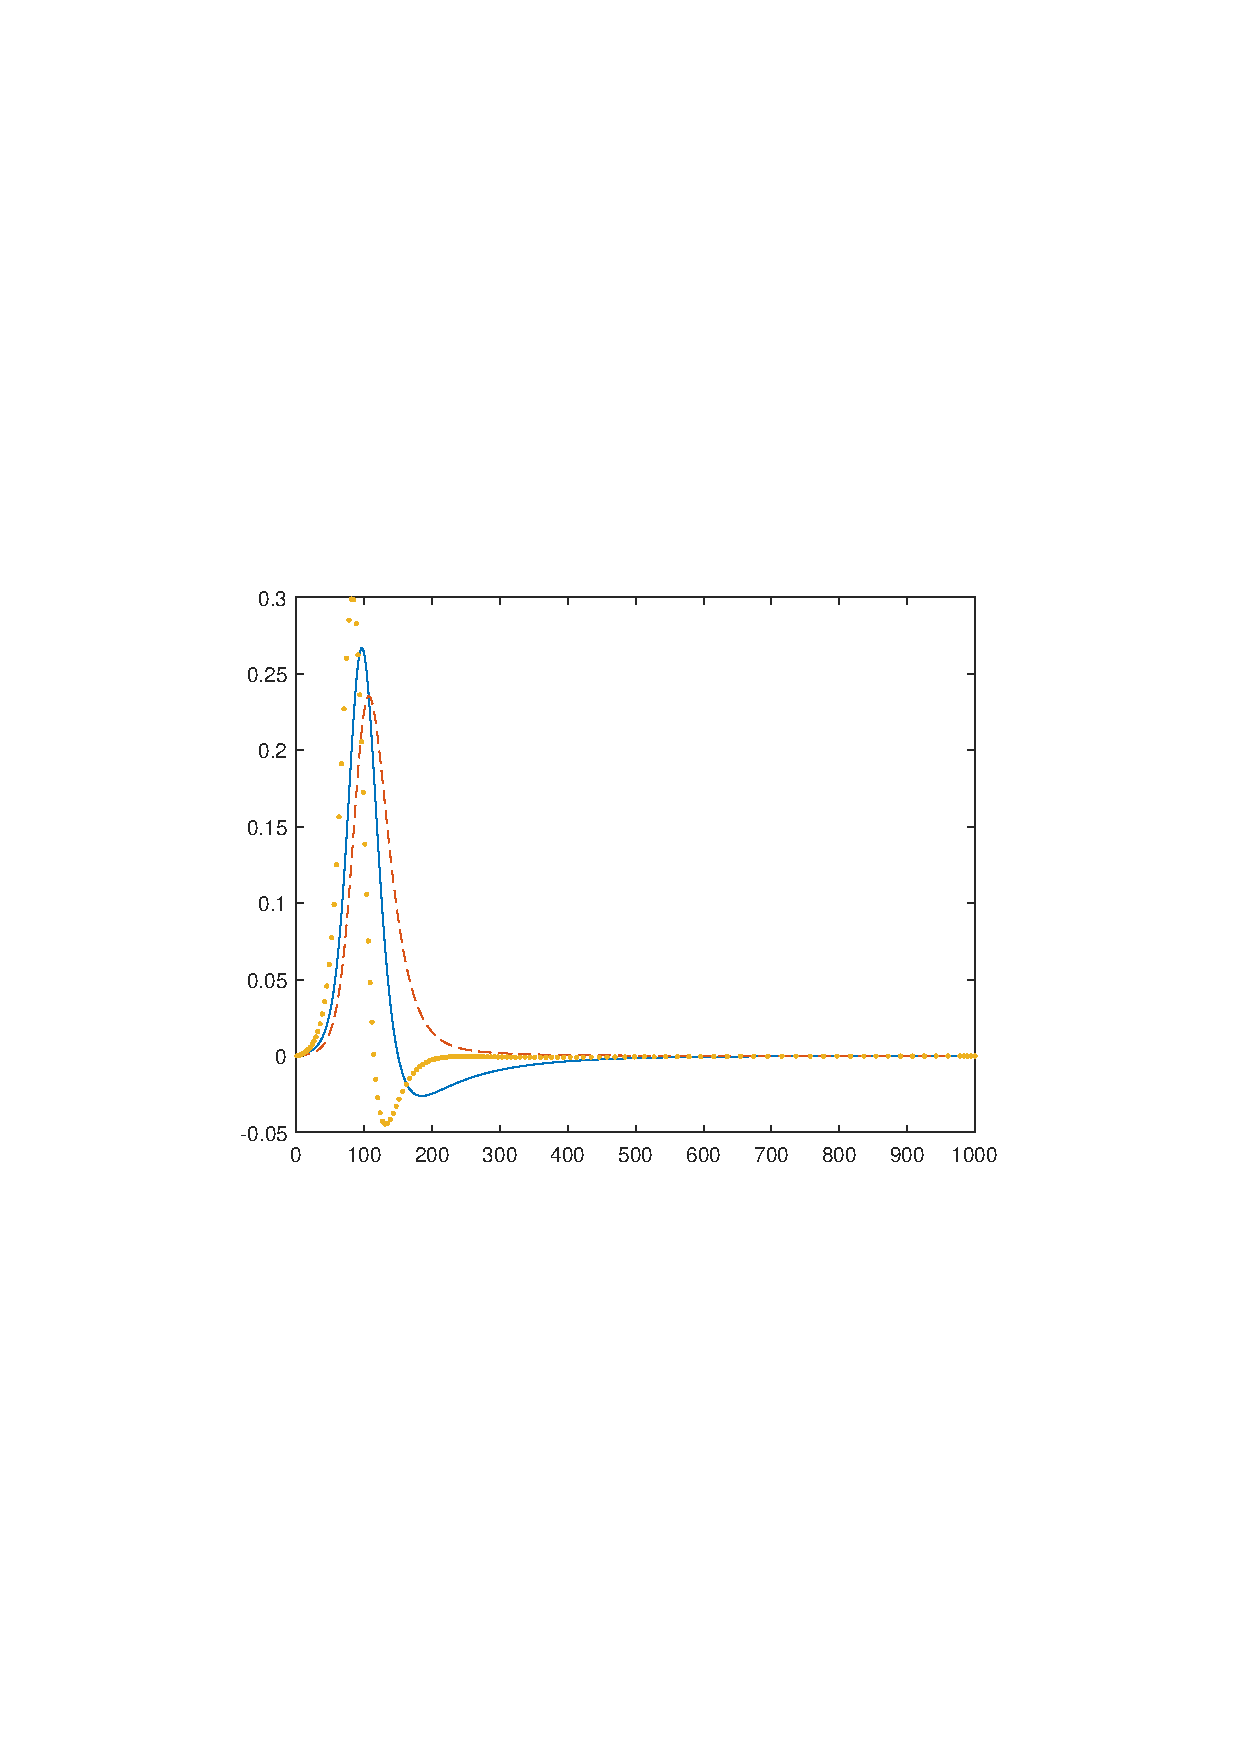
\includegraphics[width=8cm]{figures/figure_292}
  \caption{Before heightening some $\omega_{ij}$}
  \end{minipage}
  \qquad\qquad\qquad\qquad
  	\begin{minipage}[t]{0.3\textwidth}
  \centering
  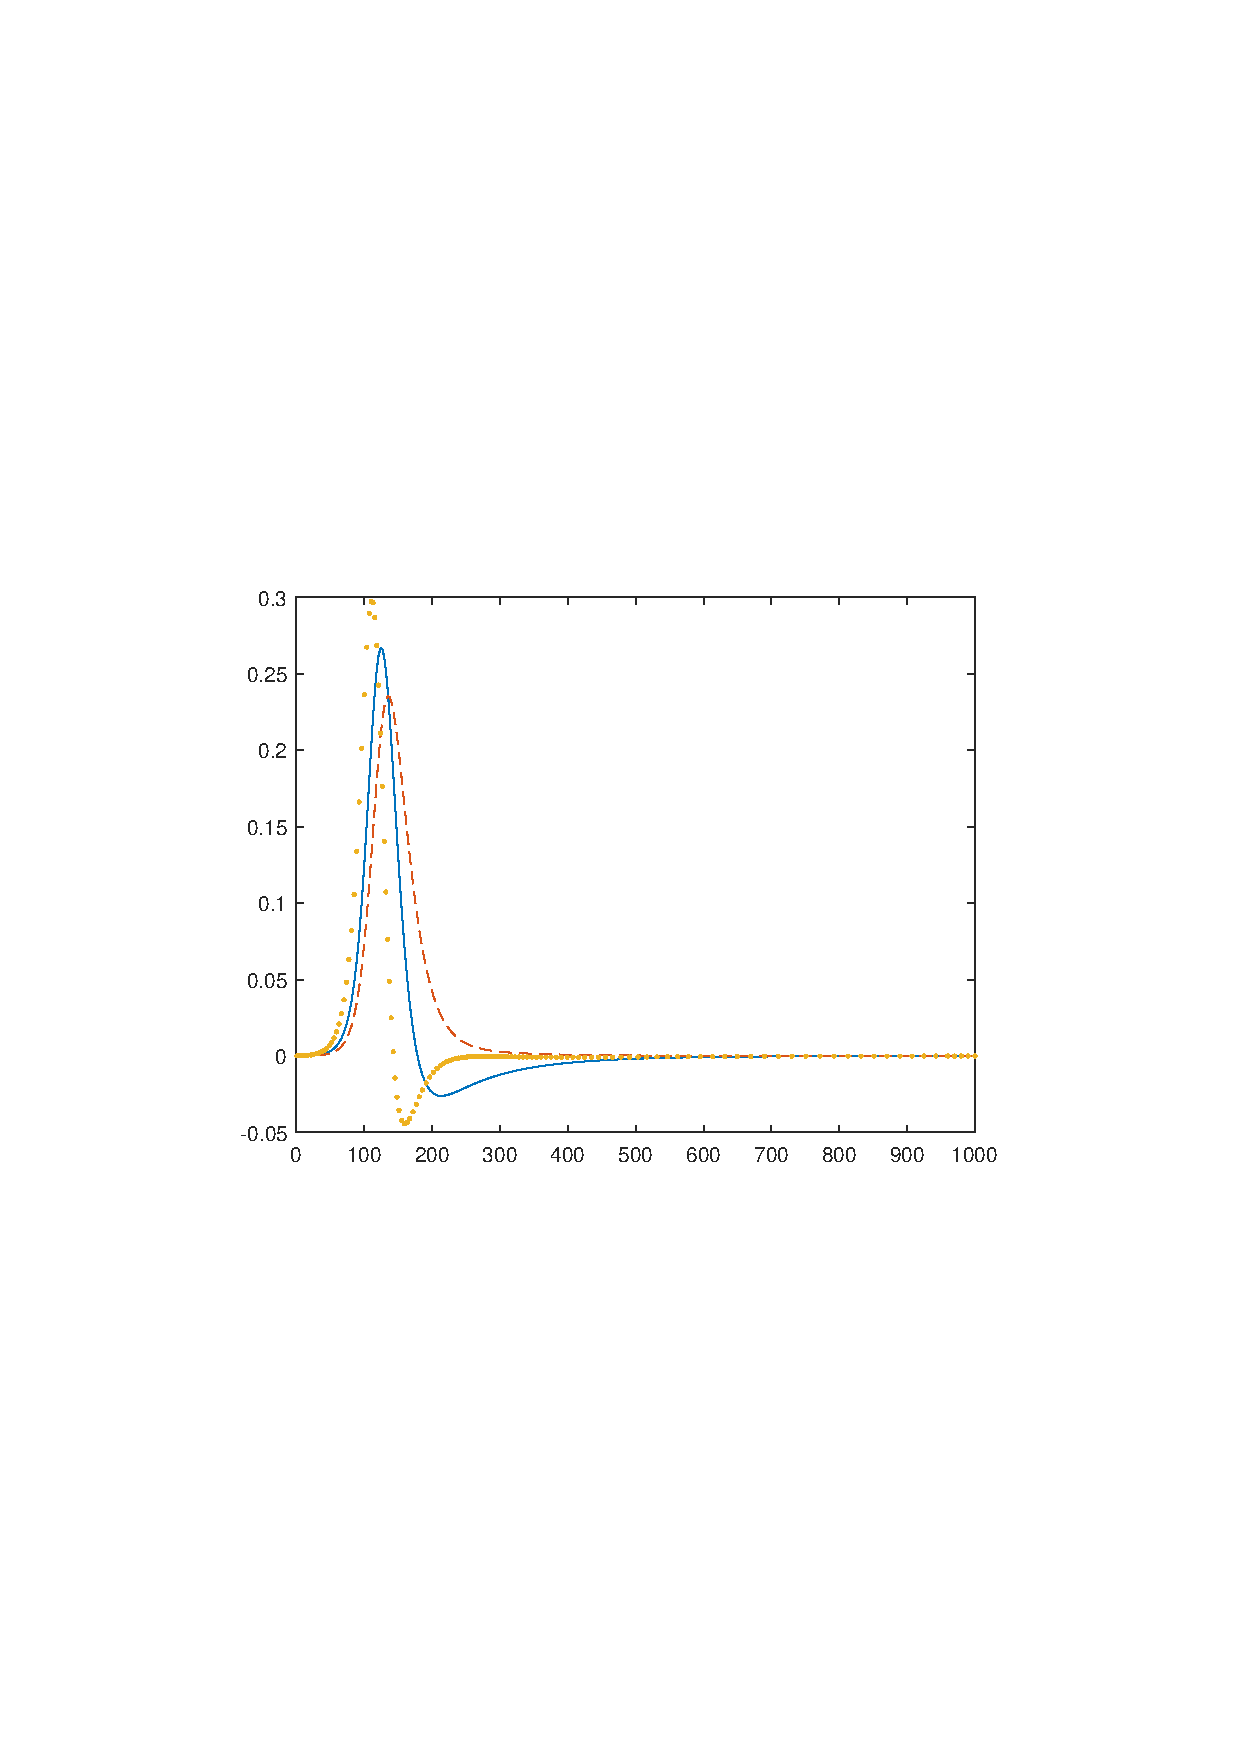
\includegraphics[width=8cm]{figures/figure_291}
  \caption{After heightening some $\omega_{ij}$}
  \end{minipage}
  \end{flushleft}
  
\end{figure}

The breakout time is delayed after making this adjustment and the situation improves even the three classes are far away from the adjusted classes. Therefore, we believe that our proposal is reasonable.





\section{Comparison \& Sensitivity Analysis}
\subsection{Model Comparison}
\begin{itemize}
	\item At first, we use the method of BP neural network to illustrate the trend and characteristic of the drug spreading. This method has kind of universality but cannot explain any internal features such as the principal of drug spreading. The result after we input the data is confusing: Reports in most of the cities keep growing steadily and in several drug abuse gathering places, the rocket toward a high level incredibly. And curves of the total 30 classes cannot give any indication about the trend for their derivative and convexity has no predictable pattern, even influenced by the errors (the errors in this panel is great because cardinal numbers are small). Also, the ratio of drug users will even reach 100\% in this case. So we made a conclusion: \textbf{Data-driven methods do not apply to our problem.}
	\item At first, we try to find the correlation of different criteria to opioid drug reports. A natural idea is to find the criteria which have higher R (Pearson correlation coefficient) when doing the linear regression. 

However, there are so many correlated criteria (37 above 0.6t), which is quite weird. Moreover, many value of R have among them have positive value in some classes and negative one in others. We explain it as the fault of value randomness. There are only 7 points to do the regression a slight error causes different results. Also, synchronous growth of reports and some criteria doesn't mean they have a causal relationship, even correlativity. In this sense, we quickly abandon this idea and take on the PSM-DiD method.
	
\end{itemize}
\subsection{Sensitivity Analysis - OAT}
Sensitivity analysis shows how the uncertainty in the output of a mathematical model or system can be apportioned to different sources of uncertainty in its input. In our model, the selected variables influencing the output value includes the drug reports statistics data classified by class from the given data, $\lambda$ (The probability of a susceptible individual becoming a drug user when meeting a drug user) and $\alpha$ (The proportion of drug users who enter treatment and recover). 

Meanwhile, in this model we use the input drug reports data to compute a reasonable $\omega_{ij}$, which indicates the drug abuse cultural exports weighting ratio of Class $i$ over Class $j$. In this section, we are going to adapt the one-at-a-time method (OAT) to analyze how a minor or major change in the input data or variable will affect the output.In this model, $Q$ (The relative residue between estimated and true new drug reports considering all years and classes) represents the difference between the actual data and the modeled result. Therefore, in this section, the change of $Q$ represents the change in the output of the model.
 
\noindent \textbf{Analysis based on the change of the input data and $\omega_{ij}$:}The unit of analysis and prediction in our model is class, which is the clustering defined in the subsection 1.3.2. In this section class, 30 is selected as the sample for the sensitivity analysis and the total drug reports data in this class over years are tripled and divided by 3 while keeping the data in other classes unchanged. 

The result displayed in the following diagrams shows that the output of our model changes greatly on such changes hence having a relatively strong sensitivity on the input value and the variable $\omega_{ij}$.

\noindent \textbf{Analysis based on the change of $\lambda$ and $\alpha$:}
In the optimized model, we adapt $\lambda = 0.01$ and $\alpha = 0.08$ as the parameter value and the optimal model has $Q = 0.02328$. We try to change the value of $\lambda$ and $\alpha$ and examine the corresponding change of $Q$. 

From the result below, we can find out that our model is more sensitive when $\lambda$ or $\alpha$ grows greater and when $\lambda$ contributes more to the output when it is greater than less.


\begin{minipage}{\textwidth}
 \begin{minipage}[t]{0.45\textwidth}
  \centering
     \makeatletter\def\@captype{table}\makeatother\caption{Changing the input data \& $\omega_{ij}$}
       \begin{tabular}{cc} 
	\toprule[1.5pt]
Input data & $Q$\\
\midrule[1pt]
Data of class 30 shrinking to $\frac{1}{3}$ & 0.2408\\
Data unchanged & 0.0233\\
Data with class 30 tripled & 0.2590\\
\bottomrule[1.5pt]
	\end{tabular}
  \end{minipage}
  \begin{minipage}[t]{0.45\textwidth}
   \centering
        \makeatletter\def\@captype{table}\makeatother\caption{Change $\lambda$ \& $\alpha$}
         \begin{tabular}{ccc}        
          \toprule[1.5pt]
Change & $\lambda$ & $\alpha$\\
\midrule[1pt]
13\% & -0.09435 & 0.30305\\
25\% & -0.08273 & 0.25043\\
50\% & -0.05922 & 0.15354\\
100\% & -0.0111 & -0.0111\\
200\% & 0.8968 & -0.25119\\
400\% & 0.31048 & -0.51736\\
800\% & 0.83887 & -0.71154\\
\bottomrule[1.5pt]
	  \end{tabular}
   \end{minipage}
\end{minipage}




\begin{figure}[htbp!]
  \begin{flushleft}
  	\begin{minipage}[t]{0.3\textwidth}
  \centering
  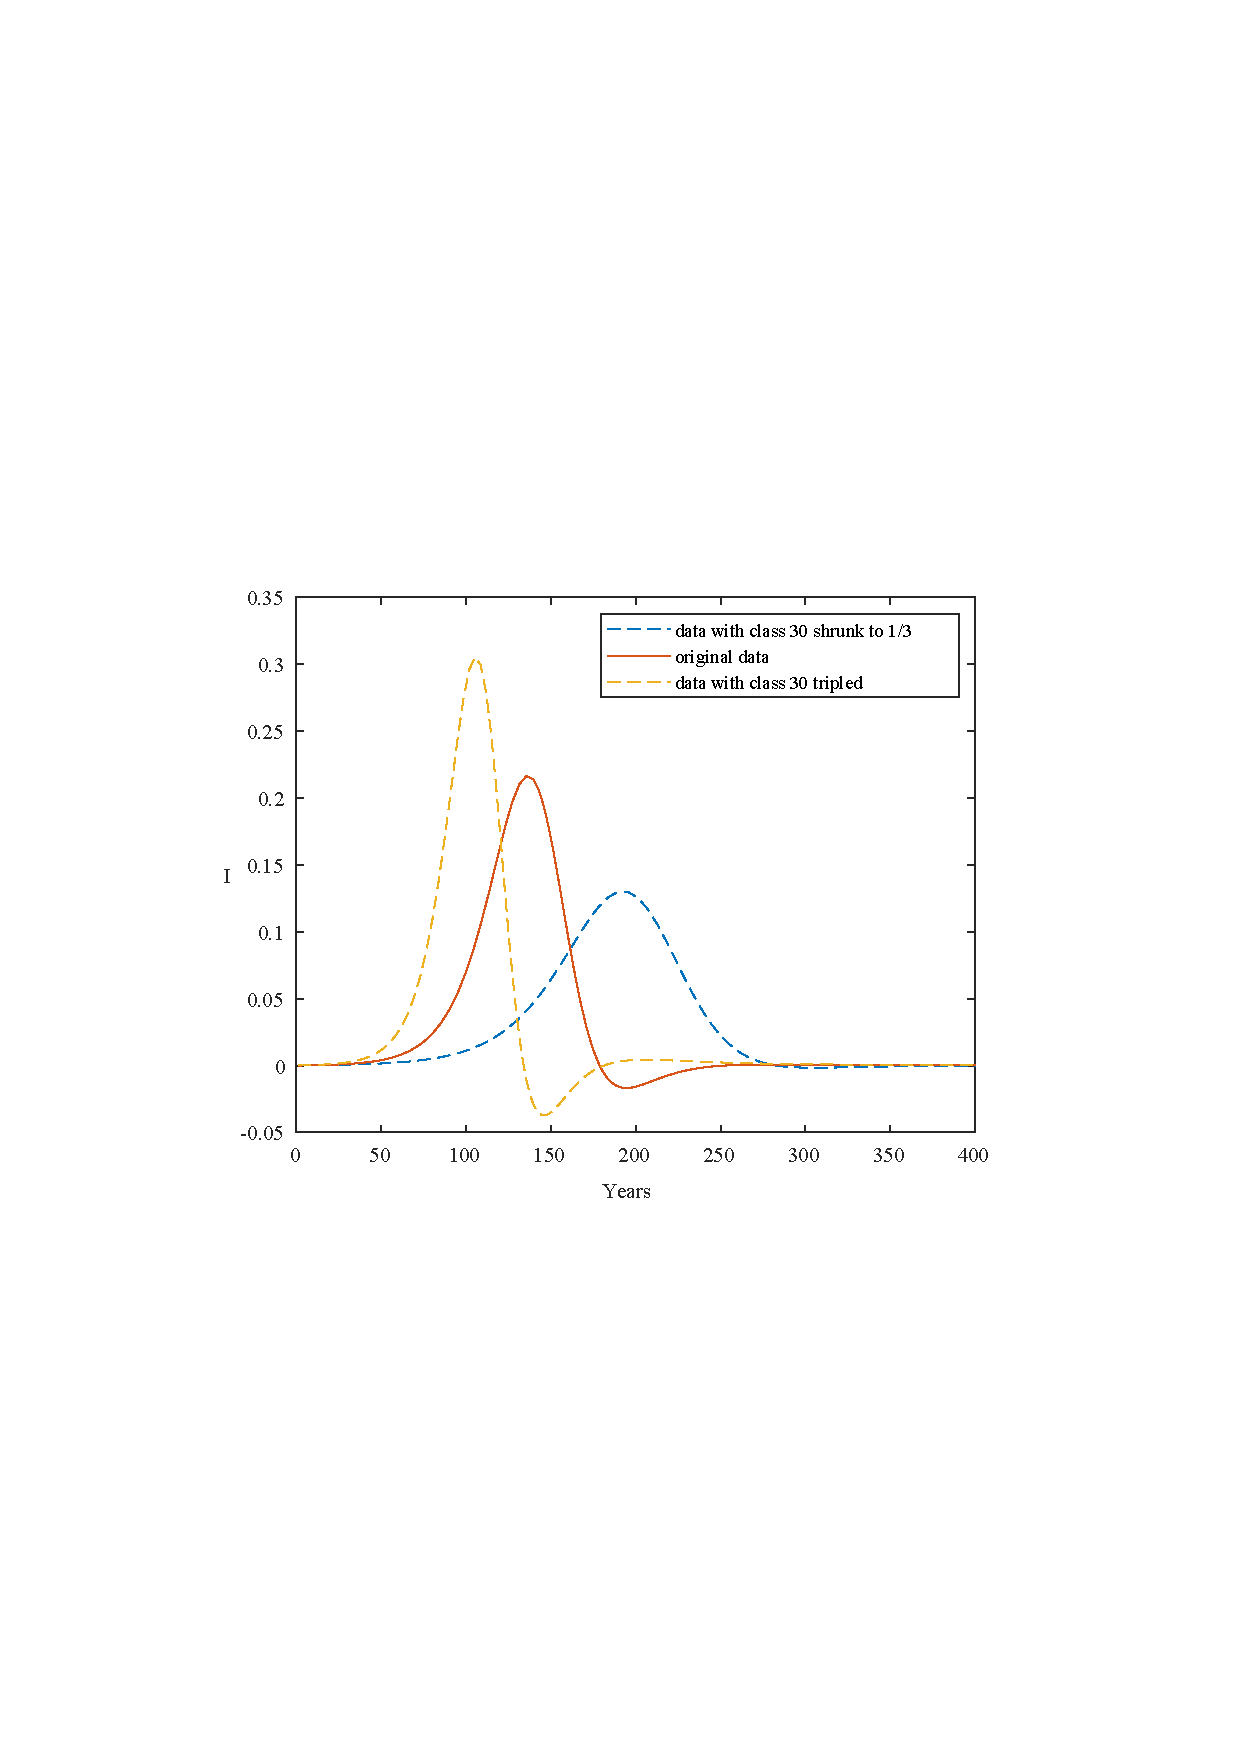
\includegraphics[width=8cm]{figures/SensitivityAnalysis1}
  \caption{Sensitivity on the change of drug report data and $\omega_{ij}$}
  \end{minipage}
  \qquad\qquad\qquad\qquad
  	\begin{minipage}[t]{0.3\textwidth}
  \centering
  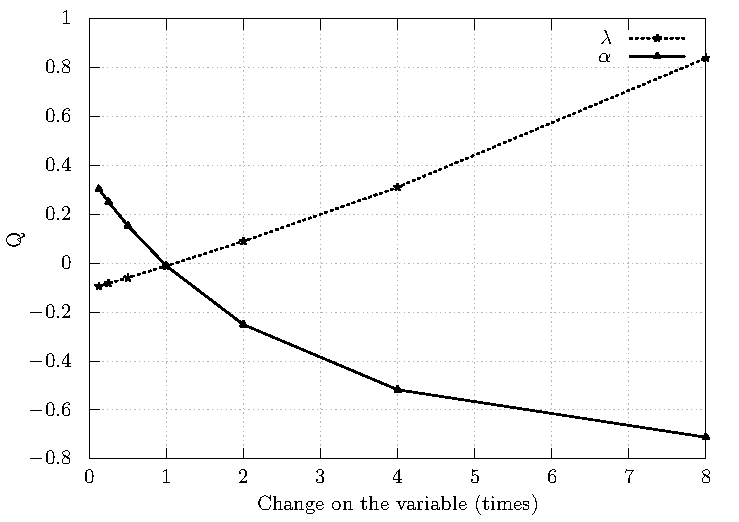
\includegraphics[width=8cm]{figures/SensitivityAnalysis2}
  \caption{Sensitivity on the change of $\lambda$ and $\alpha$}
  \end{minipage}
  \end{flushleft}
  
\end{figure}

By the way, we find that when $\alpha$ is very large, the $I_k$ may appear negative at a certain period. But in general it will not happen in reality.


\section{Evaluation \& Extension}
\subsection{Strengths}
\noindent \textbf{1. A model that feeds on data:} No matter what data one have, he/she can always test if it influences the number of drug reports in the same way. In other words, our model can refresh and keeps improving as long as new data are available.

\noindent \textbf{2. A widely-applying model:} This system can be used for many types of networks with tolerance of extreme circumstances to some extent. We also know that the selection of parameters is flexible. Moreover, the model even can solve equivalent problems about almost all kinds of drugs.

\noindent \textbf{3. Giving feasible suggestions to hinder drug abuse:} The model we establishes can give advice and reference to DEA/NFLIS about how to efficiently control the spread of opioid drug abuse.
\subsection{Weaknesses}
\noindent \textbf{1. A rough model:} When we process data with PSM-DiD and PCA methods, the method we select control group is a little rough. We can use methods considering P-value when establishing the PSM-DiD model (there exists many essays to explain this) and use data of counties for more accuracy when establishing both two models if we have more time.

\noindent \textbf{2. Arbitrage functions:} The functions of parameters $\lambda$ , $\omega_{ij}$ may have a more complicate relation with chosen socio-economy criteria.

\noindent \textbf{3. Fear of interferences:} The model may not work properly when some emergencies or implementation of policies related to some areas such as traffic and health care happen.

\subsection{Extension}
\noindent \textbf{1.} We can find better functions of parameters in the model using methods like numerical simulation \& BP neural network to decide the best function expression of $\lambda$ and $\omega_{ij}$, if we have more free time.

\noindent \textbf{2.} We can modify the SIR model in advance like adding the relapsing rate, the rate of becoming drug abhorrer and the rate of taking drugs due to local drug cartels. We can even take psychological factors into consideration.

\noindent \textbf{3.} There are many objective methods that can be combined with the AHP method to get a more proper weight between several criteria. Specialists can do a better job.

\noindent \textbf{4.} Many indicators like languages, human races can be combined into the data-integrated model, if there is more time.

\newpage
\noindent Dear Chief Administrator,

We have attached our research and modeling report to this email, but we also wish to be given the honor of briefly presenting the trends we noticed and the socio-economic factors we found that might have an impact on the trend of the number of opioid drug identifications.

Above all, from the background analysis in the Section 1.1, we have found that the circumstances on illegal opioid drug users are getting increasingly worse in recent years. The total number of opioid drug identifications in the states Ohio, Kentucky, West Virginia, Virginia, and Pennsylvania has nearly doubled in the past eight years and the percentage of opioid drug identifications in the total number of drug identifications is increasing as well. Therefore, there is urgent need of taking effective measures to cope with such circumstances. 

More specifically, we have found that clustering is a prominent phenomenon in the distribution of the number of opioid drug reports in different places. In the current situation, the area around the Bucks County in Pennsylvania, the Allegheny County in Pennsylvania, the Lorain County in Ohio, the Hamilton County in Ohio and the grand area including the counties of Bell, Harlan in Kentucky and the counties Wise and Tazewell in Virginia suffer most from the illegal opioid drugs, among which Allegheny County in Pennsylvania has the most intensive drug identifications and the area  of southern-east Kentucky and southern-west Virginia has the widest spread of opioid drugs.  With our SIR model based on the given statistics, we have predicted that the places where opioid drugs might have started in each of the five states. The result is shown as the table below:
\begin{table}[htbp!]
\centering
\begin{tabular}{cc}
\toprule[1.5pt]
State & Predicted place of origin (county)\\
\midrule[1pt]
Kentucky & Harlan\\
Ohio & Hamilton\\
Pennsylvania & Allegheny\\
Virginia & Wise\\
West Virginia & Monongalia\\
\bottomrule[1.5pt]
\end{tabular}
\end{table}

What’s more, based on our prediction of the trend and the pattern of the synthetic opioid and heroin incidents, we have some certain worries:
\begin{itemize}
	\item[1. ] The county of Allegheny in the state of Pennsylvania has the most severe circumstances among the counties and this should have passive impacts on various aspects of local society. Hence some certain effective measures should be taken to interdict the spread and deals on illegal drugs.
	\item[2. ] The situation will be out of control in 40-50 years without any interference of the government. One of the features of drug abuse is that the number of drug reports will boost towards the peak value. So we must take action to prevent that.
	\item[3. ] In the recent less than four years, there is a significant increase in the counties in the northern part of the state Ohio near the Lake Erie. The increasing speed in such places is more noticeable than other places and should be paid special attention to.
\end{itemize}

In addition to the trend of the number of drug identifications alone, we have also analyzed the relationship between a wide range of socio-economic factors and the number of drug identifications. 

Among the 150 factors provided by the census, we finally find four influential criteria in them. We have found that education level and the scale of households are two prominent factors that can affect the occurrence of drug incidents. The higher the education level is, the easier similar incidents occur. After thorough analysis, we have discovered that the education level influences the income of an individual, which lays a foundation for consuming high-priced drugs. Another criterion is the scale of households. The smaller household indicates less intact families and the family member is less likely to have a tight connection with other people. Thus, such people are easier to get into addiction. Considering such a phenomenon, we propose that more social care should be given to people without intact families. Also, we have two meaningful objective criteria for reference here.

Based on the analysis above, we tried to modify our model upon these criteria to test whether it gives a better prediction. The result of the testing shows that our proposition is reasonable and more importantly, doing positive actions related to the criteria above has greatly reduced the number of incidents of opioid drugs. Therefore, our analysis and proposal are true to the fact, and the model can be more and more accurate doing the same things given fresh data.

In the end, our proposal is to increase the cultural influence of the areas where the situation drug abuse is good. We are in full confidence that as long as the proper practice is done in the corresponding areas, the trend of the spread and growth of the number of the drug incidents can be in complete control. Hope it will be helpful for you.

Please let me know if you have any questions.
\begin{flushright}
  \begin{tabular}{r}
  Best wishes, \\
  MCM Team Members\\
  \end{tabular}
\end{flushright}
\newpage

\begin{thebibliography}{99}
\bibitem{1} Jiang, Q. (2011). Mathematic Models. Beijing: Higher Education Press.
\bibitem{2} Zhuo, J. (2018). Mathematical Modeling Method and Practice. Beijing: Higher Education Press.

\bibitem{3} White, E., \& Comiskey, C. (2007). Heroin epidemics, treatment and ODE. Mathematical Biosciences, 208:312-324.
\bibitem{4} United Nations Office on Drugs and Crime. (2005). World Drug Report. Vienna: United Nations.
\bibitem{5} Liu, Z., \& Li, C. (2006). Study on Methods of Determining Weight Coefficient of index in Comprehensive Evaluation. Chinese Health Quality, 13(2), 44-46.
\bibitem{6} \url{https://en.wikipedia.org/wiki/Compartmental_models_in_epidemiology}
\end{thebibliography}

\begin{appendices}
\section{MATLAB codes \& Specific data: K-means clustering}
\begin{table}[htbp!]
  \raggedleft

    \begin{tabular}{clllllllllllllllllllllllllllllll}
    \multicolumn{1}{l}{\textbf{Class}} & \multicolumn{31}{l}{\textbf{FIPS\_Combined}} \\
    1     & \multicolumn{31}{l}{21067;39093;42071;42079;51087} \\
    2     & \multicolumn{31}{l}{39061} \\
    3     & \multicolumn{31}{l}{42013;42081;42089;51085} \\
    4     & \multicolumn{31}{l}{39035} \\
    5     & \multicolumn{31}{l}{42003} \\
    6     & \multicolumn{31}{l}{21003;21007;21027;21031;21033;21035;21047;21059;21061;21075;21083;...;21143;21157;21145;21149;21163;21171;21177;21183;21213;21221;21227;21233} \\
    7     & \multicolumn{31}{l}{39049} \\
    8     & \multicolumn{31}{l}{42101} \\
    9     & \multicolumn{31}{l}{51001;51510;51007;51011;51025;51029;51031;51036;51037;51540;51043;......;51175;51800;51181;51183;51810;51820;51830;54027} \\
    10    & \multicolumn{31}{l}{21111;39085} \\
    11    & \multicolumn{31}{l}{39081;42001;42005;42039;42073;42085;42095;42097;42111;42121;51005;51550;51067;51083;51095;51099;51117;51125;51710;51137;51760;51165;51199;54003;54033} \\
    12    & \multicolumn{31}{l}{42011;42029;42069;42075;51153} \\
    13    & \multicolumn{31}{l}{39113} \\
    14    & \multicolumn{31}{l}{21029;21043;21081;21093;21097;21135;21159;21209;21211;39011;39031;39051;39055;39065;39073;39083;39097;39107;39117;39123;39131;39159;39161;39175;54055} \\
    15    & \multicolumn{31}{l}{21013;21019;21071;21125;21173;39003;39033;39039;39047;39091;39119;39143;39149;39167;39173;51027} \\
    16    & \multicolumn{31}{l}{21001;21005;21017;21025;21045;21051;21053;21057;21063;21077;21079;21087;21099;...;39171} \\
    17    & \multicolumn{31}{l}{42017;42021;42027;42055;42115;51019;51061;51089;51107;51171;51187} \\
    18    & \multicolumn{31}{l}{21015;39027;39053;39059;39087;39101;39139;39141;39169;42007;54107} \\
    19    & \multicolumn{31}{l}{21117;39095;39099;39155;51041;51059} \\
    20    & \multicolumn{31}{l}{42009;42015;42031;42033;42035;42037;42041;42053;42057;42067;42083;42093;42103;42105;42113;42117;42119;42123;42127;42131;51840;54037;54057;54065} \\
    21    & \multicolumn{31}{l}{42045} \\
    22    & \multicolumn{31}{l}{21151;39007;39043;39057;39165;42107;42125;51177;51179;54039} \\
    23    & \multicolumn{31}{l}{21009;21011;21041;21065;21069;21089;21115;21119;21153;21155;21161;21147;21167;21185;21197;21203;21205;21217;21235;21239;39111;39127;51035;51071;51077;54081;54099} \\
    24    & \multicolumn{31}{l}{21021;21049;21073;21095;21113;21121;21179;21193;21195;21199;21231;,,,,,,;51167;51169;51173;51191;51195;5119754011;54045;54067} \\
    25    & \multicolumn{31}{l}{21037;39023;39025} \\
    26    & \multicolumn{31}{l}{39019;39067;39075;39105;39115;39121;39163;42059;51017;51515;51021;51520;......;54051;54059;54063;54069;54075;54079;54083;54087;54093;54097;54101;54103;54109} \\
    27    & \multicolumn{31}{l}{39009;39013;39041;39077;39079;42019;42077;51013;51047;51069;51121;51770} \\
    28    & \multicolumn{31}{l}{39017;39151;39153;42043;42133} \\
    29    & \multicolumn{31}{l}{39005;39029;39045;39063;39089;39103;39109;39133;39145;42049;42051;42129;51185} \\
    30    & \multicolumn{31}{l}{42025;42047;42061;42063;42065;42087;42091;42099;42109;51003;51009;51015;51023;51033;51073;51109;51139;51143;51145;51163;51193;54029} \\
    \end{tabular}%
  \label{tab:addlabel}%
\end{table}%
\textcolor[rgb]{0.98,0.00,0.00}{\textbf{MATLAB codes:}}
\lstinputlisting[language=Matlab]{./code/kmeans1.m}


\section{PCA result - 2016 Socio-economy data}
% Table generated by Excel2LaTeX from sheet 'Sheet1'
\begin{table}[htbp]
  \centering
    \begin{tabular}{|r|r|r|r|r|r|}
    \multicolumn{6}{c}{} \\
    \midrule
    \multicolumn{6}{|p{24em}|}{Component} \\
    \midrule
    \multicolumn{1}{|c|}{1} & \multicolumn{1}{c|}{2} & \multicolumn{1}{c|}{3} & \multicolumn{1}{c|}{4} & \multicolumn{1}{c|}{5} & \multicolumn{1}{c|}{6} \\
    \midrule
    .762  & -.167 & -.194 & -.327 & -.066 & .197 \\
    .997  & -.011 & .075  & -.005 & -.024 & .001 \\
    .993  & .034  & .094  & .038  & -.017 & -.017 \\
    .995  & .022  & .060  & .047  & -.040 & -.022 \\
    .984  & .065  & .120  & .102  & -.009 & -.023 \\
    .985  & .058  & .071  & .131  & -.023 & -.023 \\
    .993  & -.013 & .039  & -.095 & -.012 & -.033 \\
    .988  & .021  & .078  & -.076 & -.045 & -.066 \\
    .962  & -.106 & -.025 & -.236 & -.057 & .022 \\
    .954  & -.118 & .004  & -.244 & -.101 & .000 \\
    .981  & -.114 & .032  & -.105 & -.038 & .041 \\
    .979  & -.113 & .037  & -.120 & -.032 & .058 \\
    .978  & -.062 & .143  & -.090 & .041  & .052 \\
    .996  & .027  & .054  & .027  & -.039 & -.022 \\
    .989  & -.004 & .134  & -.008 & .034  & .019 \\
    .720  & .657  & .026  & .076  & .154  & .121 \\



    \end{tabular}%
  \label{tab:addlabel}%
\end{table}%
% Table generated by Excel2LaTeX from sheet 'Sheet1'
\begin{table}[htbp]
  \centering

    \begin{tabular}{|r|r|r|r|r|r|}
    .720  & .657  & .026  & .076  & .154  & .121 \\
    .717  & .659  & .028  & .072  & .156  & .121 \\
    .998  & .008  & .055  & .007  & -.018 & -.011 \\
    .997  & -.011 & .075  & -.005 & -.024 & .001 \\
    .984  & .065  & .120  & .102  & -.009 & -.023 \\
    .998  & .003  & .035  & .000  & -.018 & -.010 \\
    .976  & .005  & -.140 & -.155 & .015  & -.005 \\
    .981  & -.066 & -.034 & -.076 & -.056 & -.064 \\
    .981  & -.080 & .106  & -.077 & -.061 & -.057 \\
    .997  & .020  & .067  & .014  & -.007 & -.014 \\
    .989  & -.084 & -.030 & -.095 & .004  & -.005 \\
    .986  & .067  & .105  & .095  & -.008 & -.023 \\
    .986  & .018  & -.070 & -.100 & .011  & -.045 \\
    .984  & -.002 & .134  & -.075 & .051  & .025 \\
    .971  & .098  & .183  & -.069 & -.069 & .009 \\
    .998  & -.005 & .055  & -.005 & -.010 & -.008 \\
    .969  & -.157 & -.089 & -.150 & .004  & .007 \\
    .986  & .066  & .109  & .097  & -.009 & -.023 \\
    .981  & -.001 & -.069 & -.143 & -.006 & -.037 \\
    .986  & -.008 & .123  & -.076 & .049  & .032 \\
    .984  & .017  & .109  & -.072 & -.102 & .007 \\
    .979  & .041  & .037  & -.056 & .068  & -.025 \\
    .892  & -.095 & -.022 & -.380 & .087  & -.032 \\
    .695  & .686  & .022  & .050  & .148  & .119 \\
    .679  & .699  & .046  & .039  & .165  & .121 \\
    .545  & .758  & .063  & .019  & .209  & .181 \\
    .685  & .691  & .039  & .052  & .164  & .124 \\
    .752  & .614  & .022  & .087  & .141  & .117 \\
    .990  & .071  & -.037 & -.101 & -.007 & -.024 \\
    .961  & .162  & .025  & -.208 & -.048 & .008 \\
    .953  & .167  & .050  & -.168 & -.112 & -.064 \\
    .957  & .153  & .039  & -.200 & -.020 & .017 \\
    .955  & .170  & .031  & -.200 & -.065 & .026 \\
    .956  & .158  & .002  & -.234 & -.022 & .031 \\
    .961  & .162  & .025  & -.208 & -.048 & .008 \\
    .954  & .108  & -.029 & -.268 & -.039 & .017 \\
    .956  & .231  & .087  & -.132 & -.042 & -.004 \\
    .998  & -.010 & .025  & -.003 & -.031 & -.022 \\
    .996  & -.038 & .005  & .014  & -.031 & -.010 \\
    .995  & .043  & .030  & .007  & -.055 & -.027 \\
    .996  & .025  & .052  & .018  & -.033 & -.024 \\
    .997  & .003  & .047  & .005  & -.023 & -.001 \\
    .986  & -.077 & -.030 & -.046 & -.031 & -.037 \\
    .997  & .010  & .067  & .017  & -.010 & -.004 \\
    .950  & .258  & -.080 & -.062 & .104  & .004 \\
    .973  & .086  & .007  & -.197 & .049  & -.009 \\
    .966  & .044  & .210  & -.083 & .061  & -.057 \\
    .990  & .018  & .083  & -.024 & -.082 & .011 \\
    .980  & -.020 & .172  & .031  & -.042 & -.020 \\
    .981  & -.077 & -.014 & .157  & -.062 & .017 \\
    .975  & -.051 & -.078 & .177  & -.033 & .052 \\
    \end{tabular}%
  \label{tab:addlabel}%
\end{table}%
% Table generated by Excel2LaTeX from sheet 'Sheet1'
\begin{table}[htbp]
  \centering
    \begin{tabular}{|r|r|r|r|r|r|}
    .981  & .067  & .138  & .030  & -.024 & -.038 \\
    .998  & .004  & .055  & .006  & -.015 & -.012 \\
    .974  & .082  & .110  & -.169 & .030  & .020 \\
    .997  & .021  & .041  & .007  & -.034 & -.023 \\
    .967  & -.010 & .122  & -.187 & -.026 & -.042 \\
    .999  & -.001 & .043  & .004  & -.019 & -.013 \\
    .958  & .117  & .085  & -.235 & .021  & .024 \\
    .988  & .002  & .138  & .011  & .037  & .012 \\
    .982  & .054  & .139  & -.080 & .052  & .026 \\
    .998  & .010  & .057  & .005  & -.014 & -.013 \\
    .997  & .012  & .059  & .015  & -.001 & -.009 \\
    .984  & .002  & .053  & -.066 & -.101 & -.041 \\
    .933  & -.166 & .070  & -.188 & -.162 & -.014 \\
    .973  & .155  & .035  & .050  & -.040 & -.063 \\
    .963  & .182  & .081  & .064  & -.048 & -.078 \\
    .977  & .114  & -.036 & .029  & -.027 & -.039 \\
    .973  & -.043 & -.189 & .055  & -.009 & -.015 \\
    .998  & .010  & .056  & .005  & -.014 & -.014 \\
    .994  & .017  & .098  & -.012 & -.013 & -.020 \\
    .994  & .021  & .105  & -.010 & -.017 & -.018 \\
    .977  & -.038 & .177  & -.074 & .004  & -.007 \\
    .980  & .118  & -.018 & .096  & -.052 & -.036 \\
    .908  & -.174 & -.265 & -.111 & .180  & -.121 \\
    .958  & -.043 & -.248 & .127  & -.020 & .035 \\
    .958  & -.043 & -.248 & .127  & -.020 & .035 \\
    .958  & -.058 & -.238 & .124  & -.007 & .059 \\
    .956  & -.029 & -.256 & .130  & -.032 & .012 \\
    .960  & -.060 & -.252 & .098  & .005  & .015 \\
    .908  & -.174 & -.265 & -.111 & .180  & -.121 \\
    .839  & -.245 & -.304 & -.103 & .258  & -.139 \\
    .909  & -.172 & -.264 & -.111 & .178  & -.121 \\
    .958  & -.043 & -.248 & .127  & -.020 & .035 \\
    .938  & -.102 & -.292 & .072  & -.011 & .061 \\
    .958  & -.041 & -.246 & .129  & -.020 & .034 \\
    .958  & -.043 & -.248 & .127  & -.020 & .035 \\
    .914  & -.276 & -.174 & .012  & .075  & .169 \\
    .956  & -.025 & -.240 & .138  & -.024 & .062 \\
    .879  & -.035 & -.352 & .153  & -.208 & .035 \\
    .952  & -.013 & -.214 & .092  & .011  & .039 \\
    .951  & .021  & -.254 & .139  & .005  & -.049 \\
    .970  & -.090 & -.025 & .190  & -.056 & .016 \\
    .998  & .009  & .060  & .006  & -.012 & -.012 \\
    .992  & .027  & .118  & -.006 & -.023 & -.015 \\
    .959  & -.082 & -.249 & .072  & .046  & .004 \\
    .946  & -.083 & -.296 & .038  & .054  & -.009 \\
    .943  & -.073 & -.272 & .043  & .090  & -.081 \\
    .943  & -.041 & -.272 & .070  & .067  & -.085 \\
    .961  & -.135 & -.155 & .088  & .098  & .066 \\
    .910  & -.206 & -.245 & -.041 & .162  & .086 \\
    \end{tabular}%
  \label{tab:addlabel}%
\end{table}%
% Table generated by Excel2LaTeX from sheet 'Sheet1'
\begin{table}[htbp]
  \centering
    \begin{tabular}{|r|r|r|r|r|r|}
    .951  & -.036 & -.281 & .082  & -.004 & .038 \\
    .930  & -.069 & -.341 & .010  & .028  & .034 \\
    .906  & -.086 & -.283 & .132  & -.183 & .136 \\
    .857  & -.100 & -.328 & .134  & -.251 & .109 \\
    .998  & .010  & .056  & .005  & -.014 & -.014 \\
    .879  & .424  & .093  & .038  & -.051 & -.022 \\
    .934  & -.153 & -.084 & .125  & -.091 & .209 \\
    .741  & -.367 & .346  & .020  & -.058 & .348 \\
    .970  & .011  & .031  & .207  & -.056 & -.008 \\
    .881  & .087  & .337  & .107  & .027  & -.209 \\
    .971  & .137  & .115  & .133  & -.045 & -.024 \\
    .961  & .042  & .193  & .088  & -.120 & -.067 \\
    .971  & .040  & .043  & .163  & -.039 & -.046 \\
    .874  & -.134 & .391  & .097  & -.061 & -.143 \\
    .930  & -.250 & .111  & .115  & -.057 & .034 \\
    .545  & -.527 & .513  & -.090 & -.087 & .290 \\
    .968  & -.105 & .127  & .091  & .051  & -.017 \\
    .836  & -.410 & .200  & .079  & .167  & -.001 \\
    .708  & -.443 & .143  & .211  & .319  & -.105 \\
    .974  & .044  & -.018 & .196  & -.069 & -.054 \\
    .743  & -.500 & .326  & .082  & .243  & .086 \\
    .966  & -.028 & -.125 & -.012 & .027  & -.105 \\
    .907  & -.319 & -.070 & .113  & .178  & .085 \\
    .958  & .145  & .133  & .140  & -.009 & -.003 \\
    .973  & .083  & .126  & .143  & -.060 & -.011 \\
    .376  & -.598 & .578  & .017  & .137  & .294 \\
    .893  & -.071 & -.218 & -.042 & -.266 & -.005 \\
    .935  & -.051 & .180  & .207  & -.014 & -.026 \\
    .706  & -.058 & .396  & .076  & .096  & -.324 \\
    .759  & -.539 & .025  & .045  & .280  & .152 \\
    .840  & -.217 & .292  & .215  & .057  & -.270 \\
    .737  & -.192 & -.482 & -.313 & .173  & -.075 \\
    \bottomrule
    \end{tabular}%
  \label{tab:addlabel}%
\end{table}%
\newpage
\section{MATLAB codes \& Numerical Simulation of ODE equations}
\textcolor[rgb]{0.98,0.00,0.00}{\textbf{MATLAB codes:}}
\lstinputlisting[language=Matlab]{./code/processPara.m}
\section{PSM-DiD results}
% Table generated by Excel2LaTeX from sheet '1'
\begin{table}[htbp]
  \centering

    \begin{tabular}{lrrrrrr}
          & \multicolumn{1}{l}{Edu} &       & \multicolumn{1}{l}{Household} &       & \multicolumn{1}{l}{Marital} &  \\
    Class & \multicolumn{1}{l}{Treatment} & \multicolumn{1}{l}{Control} & \multicolumn{1}{l}{Treatment} & \multicolumn{1}{l}{Control} & \multicolumn{1}{l}{Treatment} & \multicolumn{1}{l}{Control} \\
          & 1     & 5     & 2     & 5     & 1     & 22 \\
          & 4     & 19    & 3     & 7     & 5     & 19 \\
          & 8     & 7     & 6     & 22    & 11    & 26 \\
          & 11    & 26    & 9     & 17    & 12    & 21 \\
          & 12    & 22    & 13    & 19    & 17    & 3 \\
          & 24    & 6     & 15    & 20    & 24    & 6 \\
          & 27    & 17    & 16    & 26    & 27    & 17 \\
          & 28    & 20    & 21    & 10    & 28    & 20 \\
          & 29    & 14    & 23    & 14    & 29    & 4 \\
          & 30    & 18    & 25    & 18    & 30    & 8 \\
    2010-2013 & 6990  & 5401  & 3442  & 5023  & 8146  & 4079 \\
    2014-2017 & 8804  & 4033  & 3988  & 3625  & 9269  & 3051 \\
    \end{tabular}%
  \label{tab:addlabel}%
\end{table}%
% Table generated by Excel2LaTeX from sheet '1'
\begin{table}[htbp]
  \centering

    \begin{tabular}{lrrrrrr}
          & \multicolumn{1}{l}{PCA1} &       & \multicolumn{1}{l}{PCA2} &       & \multicolumn{1}{l}{PCA3} &  \\
    Class & \multicolumn{1}{l}{Treatment} & \multicolumn{1}{l}{Control} & \multicolumn{1}{l}{Treatment} & \multicolumn{1}{l}{Control} & \multicolumn{1}{l}{Treatment} & \multicolumn{1}{l}{Control} \\
          & 30    & 26    & 1     & 21    & 1     & 21 \\
          & 11    & 20    & 6     & 16    & 6     & 16 \\
          & 28    & 23    & 8     & 13    & 8     & 13 \\
          & 29    & 17    & 11    & 20    & 11    & 20 \\
          & 24    & 7     & 14    & 15    & 14    & 15 \\
          & 8     & 13    & 24    & 7     & 24    & 7 \\
          & 1     & 21    & 26    & 18    & 26    & 18 \\
          & 27    & 20    & 28    & 23    & 28    & 23 \\
          & 12    & 16    & 29    & 17    & 29    & 17 \\
          & 4     & 18    & 30    & 27    & 30    & 27 \\
    2010-2013 & 6990  & 4485  & 2770  & 4194  & 8951  & 4125 \\
    2014-2017 & 8804  & 3671  & 9716  & 4670  & 9909  & 4562 \\
    \end{tabular}%
  \label{tab:addlabel}%
\end{table}%
% Table generated by Excel2LaTeX from sheet '1'
\begin{table}[htbp]
  \centering

    \begin{tabular}{lrrrrrr}
          & \multicolumn{1}{l}{PCA4} &       & \multicolumn{1}{l}{PCA5} &       & \multicolumn{1}{l}{PCA6} &  \\
    Class & \multicolumn{1}{l}{Treatment} & \multicolumn{1}{l}{Control} & \multicolumn{1}{l}{Treatment} & \multicolumn{1}{l}{Control} & \multicolumn{1}{l}{Treatment} & \multicolumn{1}{l}{Control} \\
          & 1     & 11    & 1     & 11    & 1     & 11 \\
          & 5     & 4     & 5     & 4     & 5     & 4 \\
          & 7     & 24    & 7     & 24    & 7     & 24 \\
          & 8     & 13    & 8     & 13    & 8     & 13 \\
          & 12    & 16    & 12    & 16    & 12    & 16 \\
          & 17    & 29    & 17    & 29    & 17    & 29 \\
          & 21    & 3     & 21    & 3     & 21    & 3 \\
          & 27    & 20    & 27    & 20    & 27    & 20 \\
          & 28    & 23    & 28    & 23    & 28    & 23 \\
          & 30    & 26    & 30    & 26    & 30    & 26 \\
    2010-2013 & 6316  & 5664  & 3222  & 3270  & 7745  & 4179 \\
    2014-2017 & 7018  & 5445  & 3839  & 2939  & 9087  & 3203 \\
    \end{tabular}%
  \label{tab:addlabel}%
\end{table}%
\end{appendices}
\end{document}
